\documentclass[a4paper]{book}
\usepackage{a4wide}
\usepackage{makeidx}
\usepackage{fancyhdr}
\usepackage{graphicx}
\usepackage{multicol}
\usepackage{float}
\usepackage{textcomp}
\usepackage{alltt}
\usepackage{times}
\usepackage{ifpdf}
\ifpdf
\usepackage[pdftex,
            pagebackref=true,
            colorlinks=true,
            linkcolor=blue,
            unicode
           ]{hyperref}
\else
\usepackage[ps2pdf,
            pagebackref=true,
            colorlinks=true,
            linkcolor=blue,
            unicode
           ]{hyperref}
\usepackage{pspicture}
\fi
\usepackage[utf8]{inputenc}
\usepackage{doxygen}
\makeindex
\setcounter{tocdepth}{1}
\renewcommand{\footrulewidth}{0.4pt}
\begin{document}
\begin{titlepage}
\vspace*{7cm}
\begin{center}
{\Large Phone Firewall Reference Manual\\[1ex]\large v0.01 }\\
\vspace*{1cm}
{\large Generated by Doxygen 1.5.4}\\
\vspace*{0.5cm}
{\small Wed Jul 9 11:00:11 2008}\\
\end{center}
\end{titlepage}
\clearemptydoublepage
\pagenumbering{roman}
\tableofcontents
\clearemptydoublepage
\pagenumbering{arabic}
\chapter{Phone Firewall Data Structure Index}
\section{Phone Firewall Data Structures}
Here are the data structures with brief descriptions:\begin{CompactList}
\item\contentsline{section}{\hyperlink{structEntry}{Entry} }{\pageref{structEntry}}{}
\item\contentsline{section}{\hyperlink{structentry}{entry} (Includes all informations for an \hyperlink{structentry}{entry} )}{\pageref{structentry}}{}
\end{CompactList}

\chapter{Phone Firewall File Index}
\section{Phone Firewall File List}
Here is a list of all files with brief descriptions:\begin{CompactList}
\item\contentsline{section}{\hyperlink{libphonefirewall_8h}{libphonefirewall.h} (API of the phone firewall )}{\pageref{libphonefirewall_8h}}{}
\item\contentsline{section}{\hyperlink{pf__daemon_8c}{pf\_\-daemon.c} }{\pageref{pf__daemon_8c}}{}
\item\contentsline{section}{\hyperlink{phonefirewall__administration_8c}{phonefirewall\_\-administration.c} }{\pageref{phonefirewall__administration_8c}}{}
\item\contentsline{section}{\hyperlink{phonefirewall__search_8c}{phonefirewall\_\-search.c} }{\pageref{phonefirewall__search_8c}}{}
\end{CompactList}

\chapter{Phone Firewall Data Structure Documentation}
\hypertarget{structEntry}{
\section{Entry Struct Reference}
\label{structEntry}\index{Entry@{Entry}}
}
{\tt \#include $<$libphonefirewall.h$>$}

\subsection*{Data Fields}
\begin{CompactItemize}
\item 
int \hyperlink{structEntry_138b4e79687ff5ff6de4554db0f061fd}{country\_\-code}
\item 
int \hyperlink{structEntry_9de7b96e5b65796bd35e9dc730dcd8b3}{area\_\-code}
\item 
unsigned long long \hyperlink{structEntry_1f2177afed89936f82c130ae13fb107c}{number}
\item 
char $\ast$ \hyperlink{structEntry_272e382d3efed5f970c7939742ec9603}{name}
\item 
char $\ast$ \hyperlink{structEntry_2082cdbb815dfa8b81309cd395d32986}{reason}
\item 
int \hyperlink{structEntry_85af261b3171c257892b54a7200da061}{priority}
\end{CompactItemize}


\subsection{Detailed Description}


Definition at line 52 of file libphonefirewall.h.

\subsection{Field Documentation}
\hypertarget{structEntry_138b4e79687ff5ff6de4554db0f061fd}{
\index{Entry@{Entry}!country\_\-code@{country\_\-code}}
\index{country\_\-code@{country\_\-code}!Entry@{Entry}}
\subsubsection{\setlength{\rightskip}{0pt plus 5cm}int {\bf Entry::country\_\-code}}}
\label{structEntry_138b4e79687ff5ff6de4554db0f061fd}




Definition at line 53 of file libphonefirewall.h.

Referenced by check\_\-blacklist\_\-entry(), check\_\-whitelist\_\-entry(), and evaluate\_\-stmt().\hypertarget{structEntry_9de7b96e5b65796bd35e9dc730dcd8b3}{
\index{Entry@{Entry}!area\_\-code@{area\_\-code}}
\index{area\_\-code@{area\_\-code}!Entry@{Entry}}
\subsubsection{\setlength{\rightskip}{0pt plus 5cm}int {\bf Entry::area\_\-code}}}
\label{structEntry_9de7b96e5b65796bd35e9dc730dcd8b3}




Definition at line 54 of file libphonefirewall.h.

Referenced by check\_\-blacklist\_\-entry(), check\_\-whitelist\_\-entry(), and evaluate\_\-stmt().\hypertarget{structEntry_1f2177afed89936f82c130ae13fb107c}{
\index{Entry@{Entry}!number@{number}}
\index{number@{number}!Entry@{Entry}}
\subsubsection{\setlength{\rightskip}{0pt plus 5cm}unsigned long long {\bf Entry::number}}}
\label{structEntry_1f2177afed89936f82c130ae13fb107c}




Definition at line 55 of file libphonefirewall.h.

Referenced by check\_\-blacklist\_\-entry(), check\_\-whitelist\_\-entry(), and evaluate\_\-stmt().\hypertarget{structEntry_272e382d3efed5f970c7939742ec9603}{
\index{Entry@{Entry}!name@{name}}
\index{name@{name}!Entry@{Entry}}
\subsubsection{\setlength{\rightskip}{0pt plus 5cm}char$\ast$ {\bf Entry::name}}}
\label{structEntry_272e382d3efed5f970c7939742ec9603}




Definition at line 56 of file libphonefirewall.h.\hypertarget{structEntry_2082cdbb815dfa8b81309cd395d32986}{
\index{Entry@{Entry}!reason@{reason}}
\index{reason@{reason}!Entry@{Entry}}
\subsubsection{\setlength{\rightskip}{0pt plus 5cm}char$\ast$ {\bf Entry::reason}}}
\label{structEntry_2082cdbb815dfa8b81309cd395d32986}




Definition at line 57 of file libphonefirewall.h.\hypertarget{structEntry_85af261b3171c257892b54a7200da061}{
\index{Entry@{Entry}!priority@{priority}}
\index{priority@{priority}!Entry@{Entry}}
\subsubsection{\setlength{\rightskip}{0pt plus 5cm}int {\bf Entry::priority}}}
\label{structEntry_85af261b3171c257892b54a7200da061}




Definition at line 58 of file libphonefirewall.h.

Referenced by check\_\-blacklist\_\-entry(), check\_\-whitelist\_\-entry(), and evaluate\_\-stmt().

The documentation for this struct was generated from the following file:\begin{CompactItemize}
\item 
\hyperlink{libphonefirewall_8h}{libphonefirewall.h}\end{CompactItemize}

\hypertarget{structentry}{
\section{entry Struct Reference}
\label{structentry}\index{entry@{entry}}
}
Includes all informations for an \hyperlink{structentry}{entry}.  


{\tt \#include $<$libphonefirewall.h$>$}

\subsection*{Data Fields}
\begin{CompactItemize}
\item 
int \hyperlink{structentry_c226bdbc2ae976e6287e0f76d5346bff}{country\_\-code}
\item 
int \hyperlink{structentry_0e8fbe135bf7735f8675b6829ac943c3}{area\_\-code}
\item 
unsigned long long \hyperlink{structentry_ba7411d38f6779700ca594ebb2db3201}{number}
\item 
char $\ast$ \hyperlink{structentry_ef8962564a1a313a7ddc320bb4ed739c}{name}
\item 
char $\ast$ \hyperlink{structentry_1bcaeeed116744379db6ff5c671856a2}{reason}
\item 
int \hyperlink{structentry_65a11c5accccc3ac72247a12d53098d1}{priority}
\end{CompactItemize}


\subsection{Detailed Description}
Includes all informations for an \hyperlink{structentry}{entry}. 

The struct which includes all information about entries (black- and whitelist). 

Definition at line 43 of file libphonefirewall.h.

\subsection{Field Documentation}
\hypertarget{structentry_c226bdbc2ae976e6287e0f76d5346bff}{
\index{entry@{entry}!country\_\-code@{country\_\-code}}
\index{country\_\-code@{country\_\-code}!entry@{entry}}
\subsubsection{\setlength{\rightskip}{0pt plus 5cm}int {\bf entry::country\_\-code}}}
\label{structentry_c226bdbc2ae976e6287e0f76d5346bff}




Definition at line 44 of file libphonefirewall.h.\hypertarget{structentry_0e8fbe135bf7735f8675b6829ac943c3}{
\index{entry@{entry}!area\_\-code@{area\_\-code}}
\index{area\_\-code@{area\_\-code}!entry@{entry}}
\subsubsection{\setlength{\rightskip}{0pt plus 5cm}int {\bf entry::area\_\-code}}}
\label{structentry_0e8fbe135bf7735f8675b6829ac943c3}




Definition at line 45 of file libphonefirewall.h.\hypertarget{structentry_ba7411d38f6779700ca594ebb2db3201}{
\index{entry@{entry}!number@{number}}
\index{number@{number}!entry@{entry}}
\subsubsection{\setlength{\rightskip}{0pt plus 5cm}unsigned long long {\bf entry::number}}}
\label{structentry_ba7411d38f6779700ca594ebb2db3201}




Definition at line 46 of file libphonefirewall.h.\hypertarget{structentry_ef8962564a1a313a7ddc320bb4ed739c}{
\index{entry@{entry}!name@{name}}
\index{name@{name}!entry@{entry}}
\subsubsection{\setlength{\rightskip}{0pt plus 5cm}char$\ast$ {\bf entry::name}}}
\label{structentry_ef8962564a1a313a7ddc320bb4ed739c}




Definition at line 47 of file libphonefirewall.h.\hypertarget{structentry_1bcaeeed116744379db6ff5c671856a2}{
\index{entry@{entry}!reason@{reason}}
\index{reason@{reason}!entry@{entry}}
\subsubsection{\setlength{\rightskip}{0pt plus 5cm}char$\ast$ {\bf entry::reason}}}
\label{structentry_1bcaeeed116744379db6ff5c671856a2}




Definition at line 48 of file libphonefirewall.h.\hypertarget{structentry_65a11c5accccc3ac72247a12d53098d1}{
\index{entry@{entry}!priority@{priority}}
\index{priority@{priority}!entry@{entry}}
\subsubsection{\setlength{\rightskip}{0pt plus 5cm}int {\bf entry::priority}}}
\label{structentry_65a11c5accccc3ac72247a12d53098d1}




Definition at line 49 of file libphonefirewall.h.

The documentation for this struct was generated from the following file:\begin{CompactItemize}
\item 
\hyperlink{libphonefirewall_8h}{libphonefirewall.h}\end{CompactItemize}

\chapter{Phone Firewall File Documentation}
\hypertarget{libphonefirewall_8h}{
\section{libphonefirewall.h File Reference}
\label{libphonefirewall_8h}\index{libphonefirewall.h@{libphonefirewall.h}}
}
API of the phone firewall. 



This graph shows which files directly or indirectly include this file:\nopagebreak
\begin{figure}[H]
\begin{center}
\leavevmode
\includegraphics[width=104pt]{libphonefirewall_8h__dep__incl}
\end{center}
\end{figure}
\subsection*{Defines}
\begin{CompactItemize}
\item 
\#define \hyperlink{libphonefirewall_8h_f0f2173e3b202ddf5756531b4471dcb2}{MAX\_\-LINE\_\-LENGTH}~512
\end{CompactItemize}
\subsection*{Functions}
\begin{CompactItemize}
\item 
int \hyperlink{libphonefirewall_8h_36847ed3459e2a89038772ece42a017d}{add\_\-blacklist\_\-entry} (int country\_\-code, int area\_\-code, unsigned long long number, char $\ast$name, char $\ast$reason, int priority)
\item 
int \hyperlink{libphonefirewall_8h_e6c567f38aaa0eaa9db3eb13e32cdbbd}{rm\_\-blacklist\_\-entry} (unsigned long long number)
\item 
char $\ast$ \hyperlink{libphonefirewall_8h_651cdd0245f20256305b40f13bb9df2d}{check\_\-blacklist\_\-entry} (int country\_\-code, int area\_\-code, unsigned long long number, int priority)
\item 
int \hyperlink{libphonefirewall_8h_eec16cb88eb546b1a2490e6716d75f8b}{add\_\-whitelist\_\-entry} (int country\_\-code, int area\_\-code, unsigned long long number, char $\ast$name, char $\ast$reason, int priority)
\item 
int \hyperlink{libphonefirewall_8h_e8a4ee30cf26b05a55680dc3a972f1a4}{rm\_\-whitelist\_\-entry} (unsigned long long number)
\item 
char $\ast$ \hyperlink{libphonefirewall_8h_032c45d6c7830492ddeaa8cabfc845c3}{check\_\-whitelist\_\-entry} (int country\_\-code, int area\_\-code, unsigned long long number, int priority)
\end{CompactItemize}


\subsection{Detailed Description}
API of the phone firewall. 

\begin{Desc}
\item[Author:]Alex Oberhauser\end{Desc}
The header file of the Phone Firewall. Blocks or accepts incoming phone calls, so it's possible to prevent disturbing phone calls. Provides a API which can used by other application to build nice programs.

Implemented for the OpenMoko framework. 

Definition in file \hyperlink{libphonefirewall_8h-source}{libphonefirewall.h}.

\subsection{Define Documentation}
\hypertarget{libphonefirewall_8h_f0f2173e3b202ddf5756531b4471dcb2}{
\index{libphonefirewall.h@{libphonefirewall.h}!MAX\_\-LINE\_\-LENGTH@{MAX\_\-LINE\_\-LENGTH}}
\index{MAX\_\-LINE\_\-LENGTH@{MAX\_\-LINE\_\-LENGTH}!libphonefirewall.h@{libphonefirewall.h}}
\subsubsection{\setlength{\rightskip}{0pt plus 5cm}\#define MAX\_\-LINE\_\-LENGTH~512}}
\label{libphonefirewall_8h_f0f2173e3b202ddf5756531b4471dcb2}




Definition at line 33 of file libphonefirewall.h.

Referenced by check\_\-blacklist\_\-entry(), and check\_\-whitelist\_\-entry().

\subsection{Function Documentation}
\hypertarget{libphonefirewall_8h_36847ed3459e2a89038772ece42a017d}{
\index{libphonefirewall.h@{libphonefirewall.h}!add\_\-blacklist\_\-entry@{add\_\-blacklist\_\-entry}}
\index{add\_\-blacklist\_\-entry@{add\_\-blacklist\_\-entry}!libphonefirewall.h@{libphonefirewall.h}}
\subsubsection{\setlength{\rightskip}{0pt plus 5cm}int add\_\-blacklist\_\-entry (int {\em country\_\-code}, int {\em area\_\-code}, unsigned long long {\em number}, char $\ast$ {\em name}, char $\ast$ {\em reason}, int {\em priority})}}
\label{libphonefirewall_8h_36847ed3459e2a89038772ece42a017d}


Add a number to the blacklist. The number will be blocked after that.

\begin{Desc}
\item[Parameters:]
\begin{description}
\item[{\em country\_\-code}]The country code (for example 39 for Italy, 43 for Austria, and so one) \item[{\em area\_\-code}]The area code which indicates your mobile operator. \item[{\em number}]The telephone number of the person. \item[{\em name}]The name of the person. \item[{\em reason}]Why you have blocked this person. \item[{\em priority}]Gives the entry a priority. 0 is standard. If the priority is higher the value will be also blocked/accepted if a higher priority is choosen.\end{description}
\end{Desc}
\begin{Desc}
\item[Returns:]If all goes well 0 (zero) otherwise an errno code. \end{Desc}


Definition at line 40 of file phonefirewall\_\-administration.c.

References BLACKLIST\_\-PREFIX, DELIM, filename, and set\_\-filename().

Here is the call graph for this function:\nopagebreak
\begin{figure}[H]
\begin{center}
\leavevmode
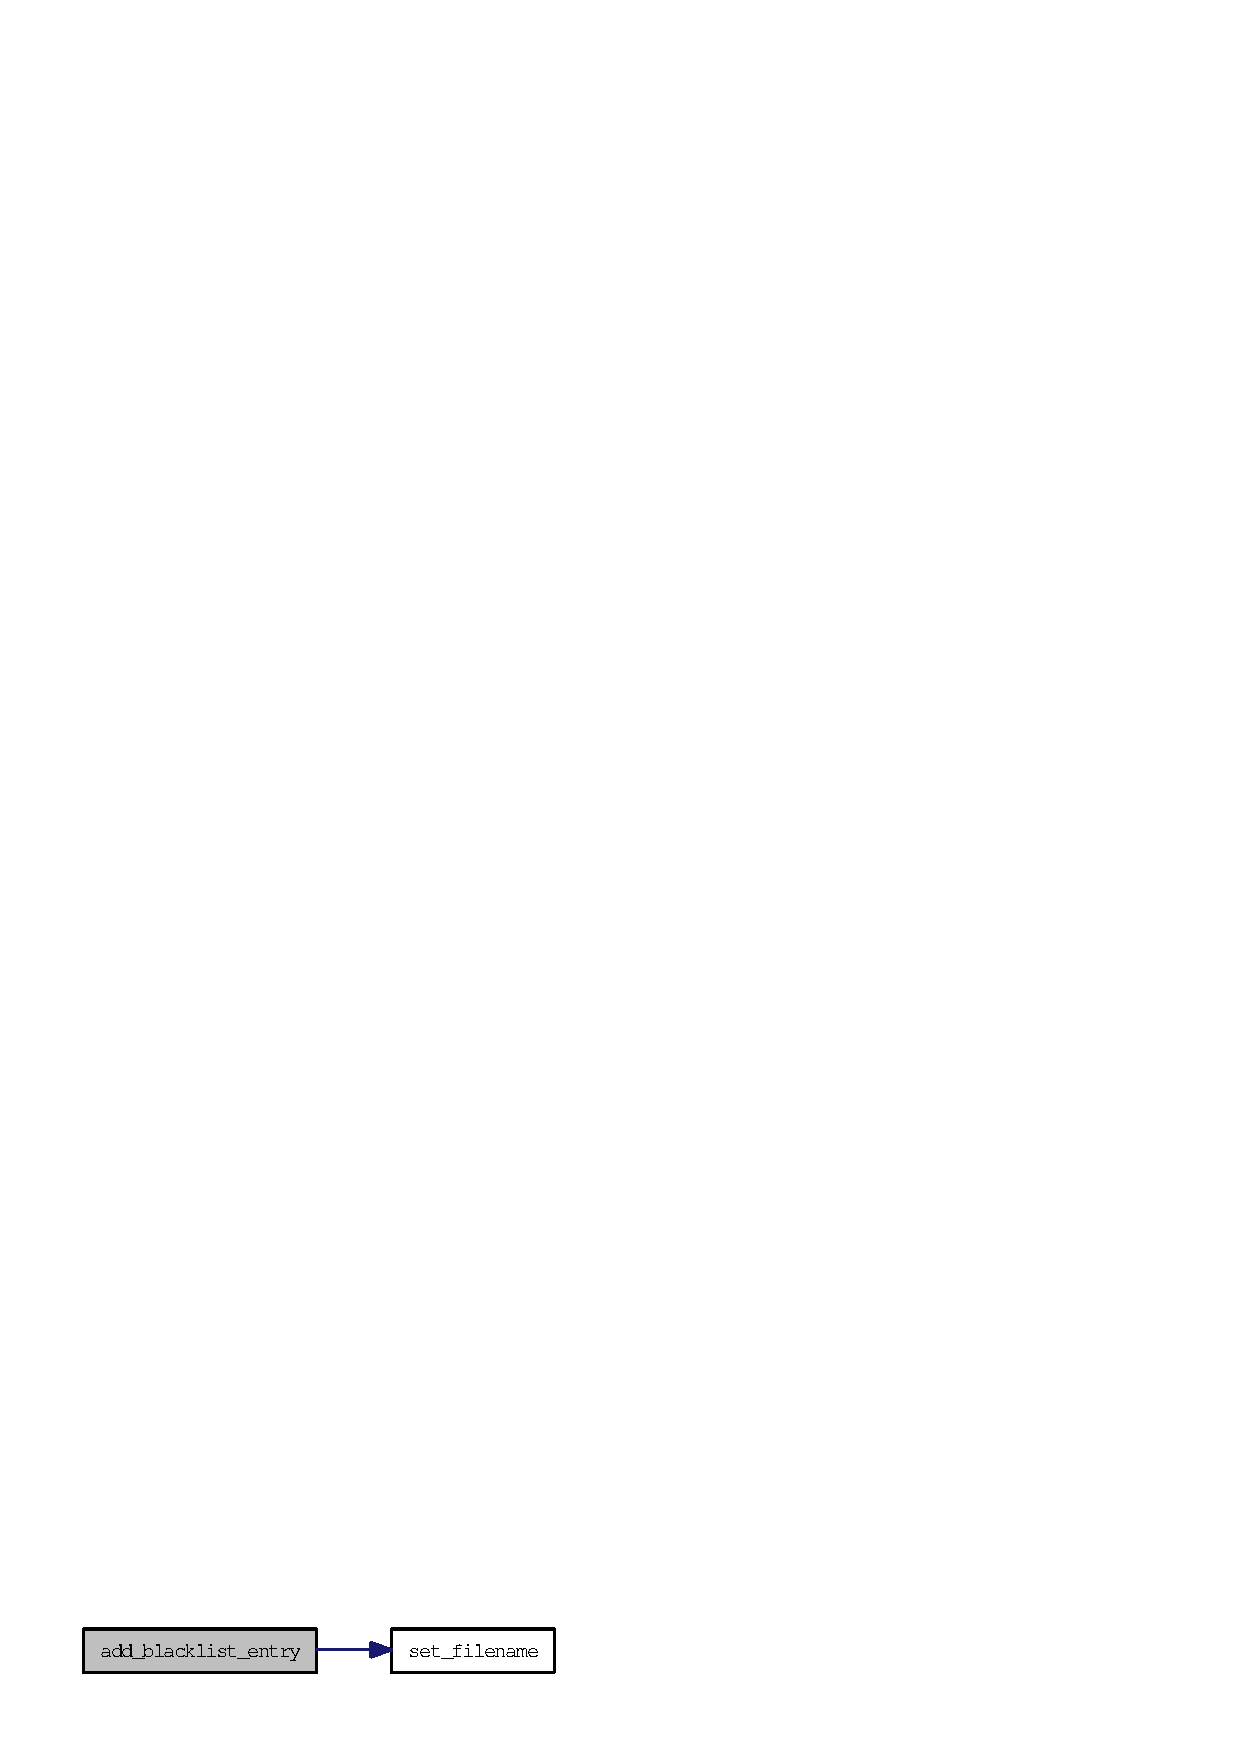
\includegraphics[width=135pt]{libphonefirewall_8h_36847ed3459e2a89038772ece42a017d_cgraph}
\end{center}
\end{figure}
\hypertarget{libphonefirewall_8h_eec16cb88eb546b1a2490e6716d75f8b}{
\index{libphonefirewall.h@{libphonefirewall.h}!add\_\-whitelist\_\-entry@{add\_\-whitelist\_\-entry}}
\index{add\_\-whitelist\_\-entry@{add\_\-whitelist\_\-entry}!libphonefirewall.h@{libphonefirewall.h}}
\subsubsection{\setlength{\rightskip}{0pt plus 5cm}int add\_\-whitelist\_\-entry (int {\em country\_\-code}, int {\em area\_\-code}, unsigned long long {\em number}, char $\ast$ {\em name}, char $\ast$ {\em reason}, int {\em priority})}}
\label{libphonefirewall_8h_eec16cb88eb546b1a2490e6716d75f8b}


Add a number to the whitelist. The number will be accepted after that.

\begin{Desc}
\item[Parameters:]
\begin{description}
\item[{\em country\_\-code}]The country code (for example 39 for Italy, 43 for Austria, and so one) \item[{\em area\_\-code}]The area code which indicates your mobile operator. \item[{\em number}]The telephone number of the person. \item[{\em name}]The name of the person. \item[{\em reason}]Why you have blocked this person. \item[{\em priority}]Gives the entry a priority. 0 is standard. If the priority is higher the value will be also blocked/accepted if a higher priority is choosen.\end{description}
\end{Desc}
\begin{Desc}
\item[Returns:]If all goes well 0 (zero) otherwise an errno code. \end{Desc}


Definition at line 53 of file phonefirewall\_\-administration.c.

References DELIM, filename, set\_\-filename(), and WHITELIST\_\-PREFIX.

Here is the call graph for this function:\nopagebreak
\begin{figure}[H]
\begin{center}
\leavevmode
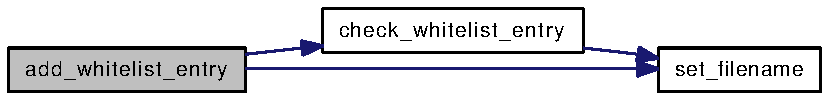
\includegraphics[width=136pt]{libphonefirewall_8h_eec16cb88eb546b1a2490e6716d75f8b_cgraph}
\end{center}
\end{figure}
\hypertarget{libphonefirewall_8h_651cdd0245f20256305b40f13bb9df2d}{
\index{libphonefirewall.h@{libphonefirewall.h}!check\_\-blacklist\_\-entry@{check\_\-blacklist\_\-entry}}
\index{check\_\-blacklist\_\-entry@{check\_\-blacklist\_\-entry}!libphonefirewall.h@{libphonefirewall.h}}
\subsubsection{\setlength{\rightskip}{0pt plus 5cm}char$\ast$ check\_\-blacklist\_\-entry (int {\em country\_\-code}, int {\em area\_\-code}, unsigned long long {\em number}, int {\em priority})}}
\label{libphonefirewall_8h_651cdd0245f20256305b40f13bb9df2d}


Checks if a number is on the blacklist.

\begin{Desc}
\item[Parameters:]
\begin{description}
\item[{\em country\_\-code}]The country code (for example 39 for Italy, 43 for Austria, and so one) \item[{\em area\_\-code}]The area code which indicates your mobile operator. \item[{\em number}]The telephone number of the person. \item[{\em priority}]Gives the entry a priority. 0 is standard. If the priority is higher the value will be also blocked/accepted if a higher priority is choosen.\end{description}
\end{Desc}
\begin{Desc}
\item[Returns:]If noting is found NULL, otherwise the number. \end{Desc}


Definition at line 74 of file phonefirewall\_\-administration.c.

References BLACKLIST\_\-PREFIX, DELIM, filename, MAX\_\-LINE\_\-LENGTH, and set\_\-filename().

Here is the call graph for this function:\nopagebreak
\begin{figure}[H]
\begin{center}
\leavevmode
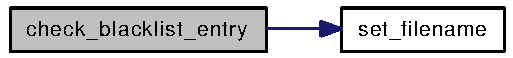
\includegraphics[width=141pt]{libphonefirewall_8h_651cdd0245f20256305b40f13bb9df2d_cgraph}
\end{center}
\end{figure}
\hypertarget{libphonefirewall_8h_032c45d6c7830492ddeaa8cabfc845c3}{
\index{libphonefirewall.h@{libphonefirewall.h}!check\_\-whitelist\_\-entry@{check\_\-whitelist\_\-entry}}
\index{check\_\-whitelist\_\-entry@{check\_\-whitelist\_\-entry}!libphonefirewall.h@{libphonefirewall.h}}
\subsubsection{\setlength{\rightskip}{0pt plus 5cm}char$\ast$ check\_\-whitelist\_\-entry (int {\em country\_\-code}, int {\em area\_\-code}, unsigned long long {\em number}, int {\em priority})}}
\label{libphonefirewall_8h_032c45d6c7830492ddeaa8cabfc845c3}


Checks if a number is on the whitelist.

\begin{Desc}
\item[Parameters:]
\begin{description}
\item[{\em country\_\-code}]The country code (for example 39 for Italy, 43 for Austria, and so one) \item[{\em area\_\-code}]The area code which indicates your mobile operator. \item[{\em number}]The telephone number of the person. \item[{\em priority}]Gives the entry a priority. 0 is standard. If the priority is higher the value will be also blocked/accepted if a higher priority is choosen.\end{description}
\end{Desc}
\begin{Desc}
\item[Returns:]If noting is found NULL, otherwise the number. \end{Desc}


Definition at line 105 of file phonefirewall\_\-administration.c.

References DELIM, filename, MAX\_\-LINE\_\-LENGTH, set\_\-filename(), and WHITELIST\_\-PREFIX.

Here is the call graph for this function:\nopagebreak
\begin{figure}[H]
\begin{center}
\leavevmode
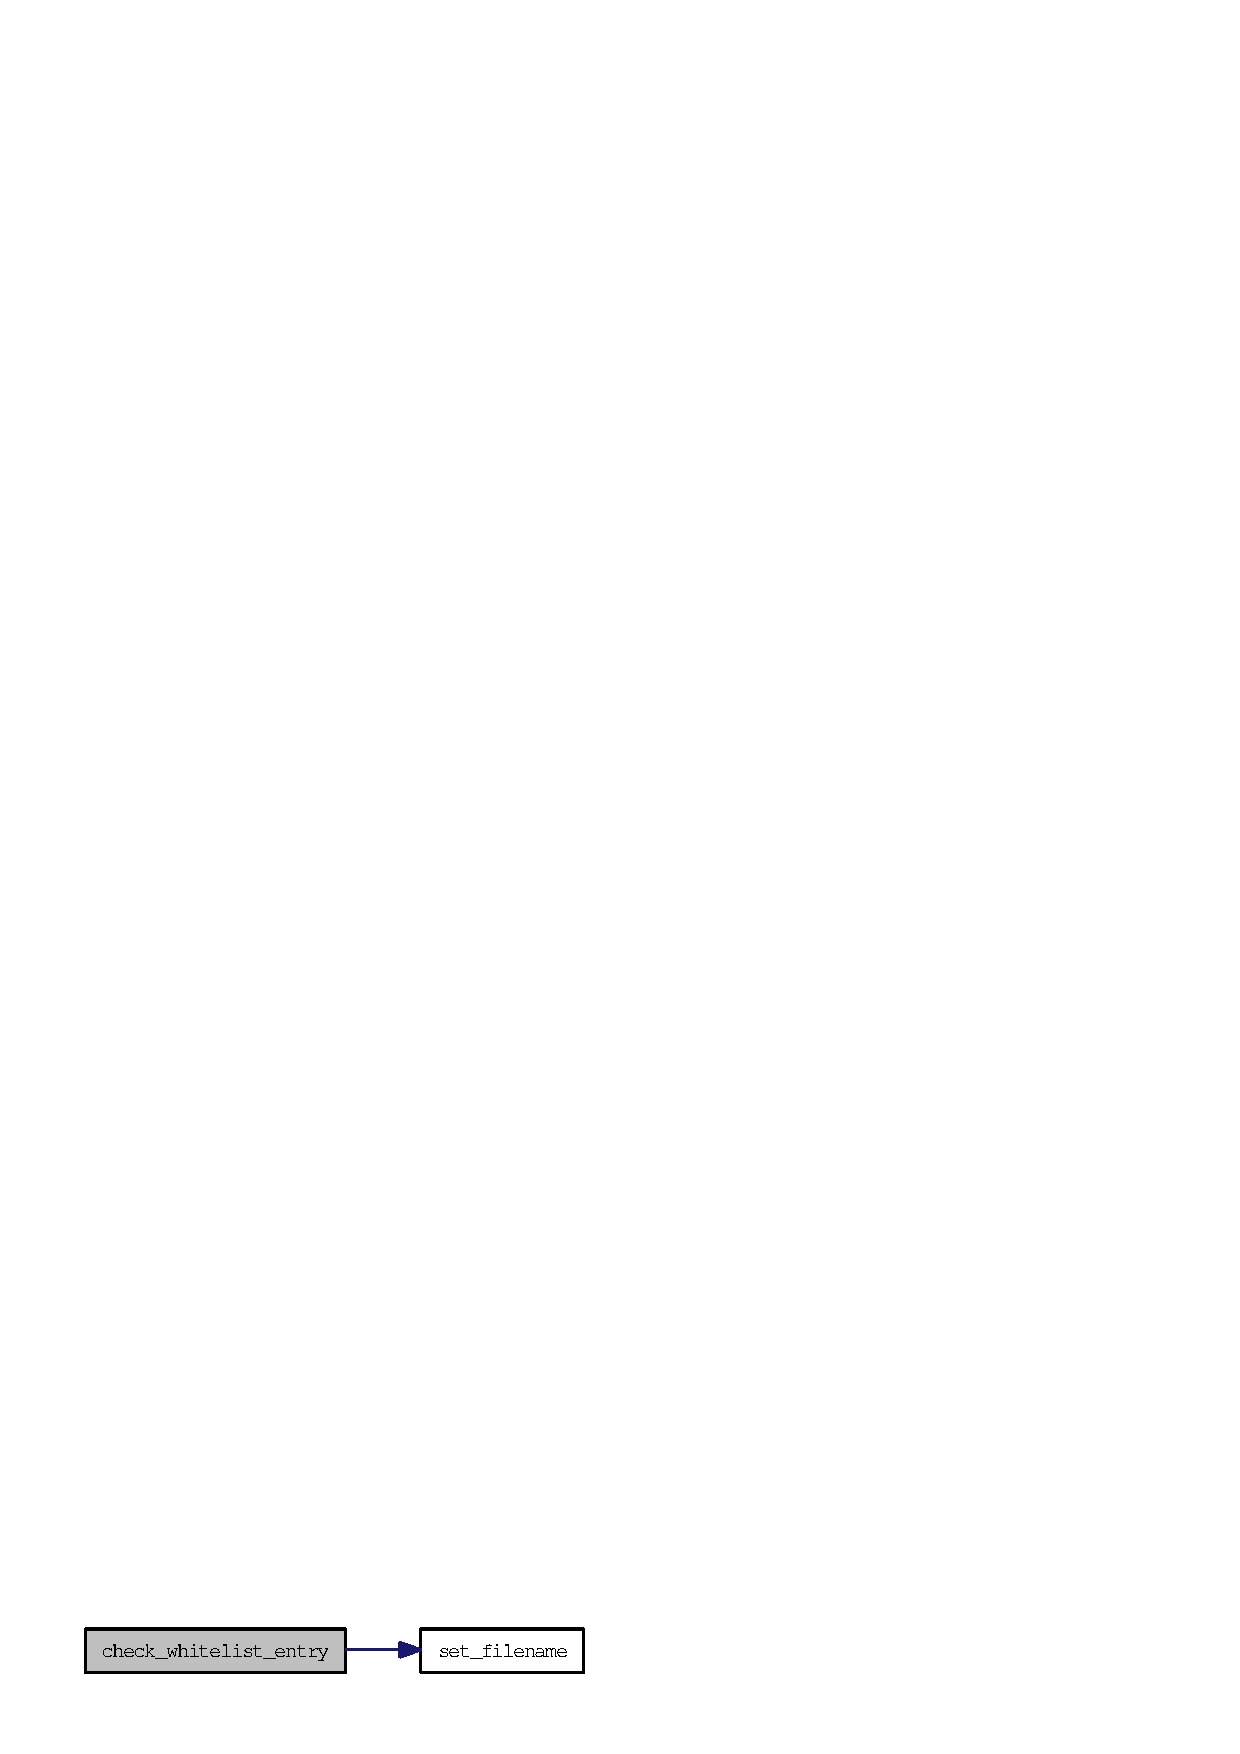
\includegraphics[width=142pt]{libphonefirewall_8h_032c45d6c7830492ddeaa8cabfc845c3_cgraph}
\end{center}
\end{figure}
\hypertarget{libphonefirewall_8h_e6c567f38aaa0eaa9db3eb13e32cdbbd}{
\index{libphonefirewall.h@{libphonefirewall.h}!rm\_\-blacklist\_\-entry@{rm\_\-blacklist\_\-entry}}
\index{rm\_\-blacklist\_\-entry@{rm\_\-blacklist\_\-entry}!libphonefirewall.h@{libphonefirewall.h}}
\subsubsection{\setlength{\rightskip}{0pt plus 5cm}int rm\_\-blacklist\_\-entry (unsigned long long {\em number})}}
\label{libphonefirewall_8h_e6c567f38aaa0eaa9db3eb13e32cdbbd}


Removes a blocked number from the blacklist.

\begin{Desc}
\item[Parameters:]
\begin{description}
\item[{\em number}]The number which will be deleted.\end{description}
\end{Desc}
\begin{Desc}
\item[Returns:]If all goes right 0, otherwise an error code. \end{Desc}


Definition at line 66 of file phonefirewall\_\-administration.c.\hypertarget{libphonefirewall_8h_e8a4ee30cf26b05a55680dc3a972f1a4}{
\index{libphonefirewall.h@{libphonefirewall.h}!rm\_\-whitelist\_\-entry@{rm\_\-whitelist\_\-entry}}
\index{rm\_\-whitelist\_\-entry@{rm\_\-whitelist\_\-entry}!libphonefirewall.h@{libphonefirewall.h}}
\subsubsection{\setlength{\rightskip}{0pt plus 5cm}int rm\_\-whitelist\_\-entry (unsigned long long {\em number})}}
\label{libphonefirewall_8h_e8a4ee30cf26b05a55680dc3a972f1a4}


Removes a accepted number from the whitelist.

\begin{Desc}
\item[Parameters:]
\begin{description}
\item[{\em number}]The number which will be deleted.\end{description}
\end{Desc}
\begin{Desc}
\item[Returns:]If all goes right 0, otherwise an error code. \end{Desc}


Definition at line 70 of file phonefirewall\_\-administration.c.
\hypertarget{logfile_8c}{
\section{logfile.c File Reference}
\label{logfile_8c}\index{logfile.c@{logfile.c}}
}
{\tt \#include $<$stdio.h$>$}\par
{\tt \#include $<$stdlib.h$>$}\par
{\tt \#include $<$time.h$>$}\par
{\tt \#include \char`\"{}logfile.h\char`\"{}}\par


Include dependency graph for logfile.c:\nopagebreak
\begin{figure}[H]
\begin{center}
\leavevmode
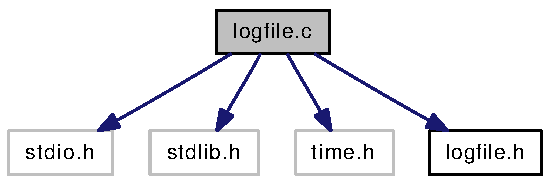
\includegraphics[width=150pt]{logfile_8c__incl}
\end{center}
\end{figure}
\subsection*{Functions}
\begin{CompactItemize}
\item 
char $\ast$ \hyperlink{logfile_8c_68a0e9d22417dfcf9c0be64261352e64}{asctime} (const struct tm $\ast$timeptr)
\item 
int \hyperlink{logfile_8c_f71f5daf2025b4e30a18ccedf7c34863}{write\_\-logentry} (char $\ast$msg, char $\ast$component, int flag)
\end{CompactItemize}


\subsection{Function Documentation}
\hypertarget{logfile_8c_68a0e9d22417dfcf9c0be64261352e64}{
\index{logfile.c@{logfile.c}!asctime@{asctime}}
\index{asctime@{asctime}!logfile.c@{logfile.c}}
\subsubsection{\setlength{\rightskip}{0pt plus 5cm}char$\ast$ asctime (const struct tm $\ast$ {\em timeptr})}}
\label{logfile_8c_68a0e9d22417dfcf9c0be64261352e64}


Compounds a humand readable date and time string.

\begin{Desc}
\item[Parameters:]
\begin{description}
\item[{\em timeptr}]A pointer to the actual time.\end{description}
\end{Desc}
\begin{Desc}
\item[Returns:]The date and time as a string. \end{Desc}


Definition at line 33 of file logfile.c.

Referenced by write\_\-logentry().

Here is the caller graph for this function:\nopagebreak
\begin{figure}[H]
\begin{center}
\leavevmode
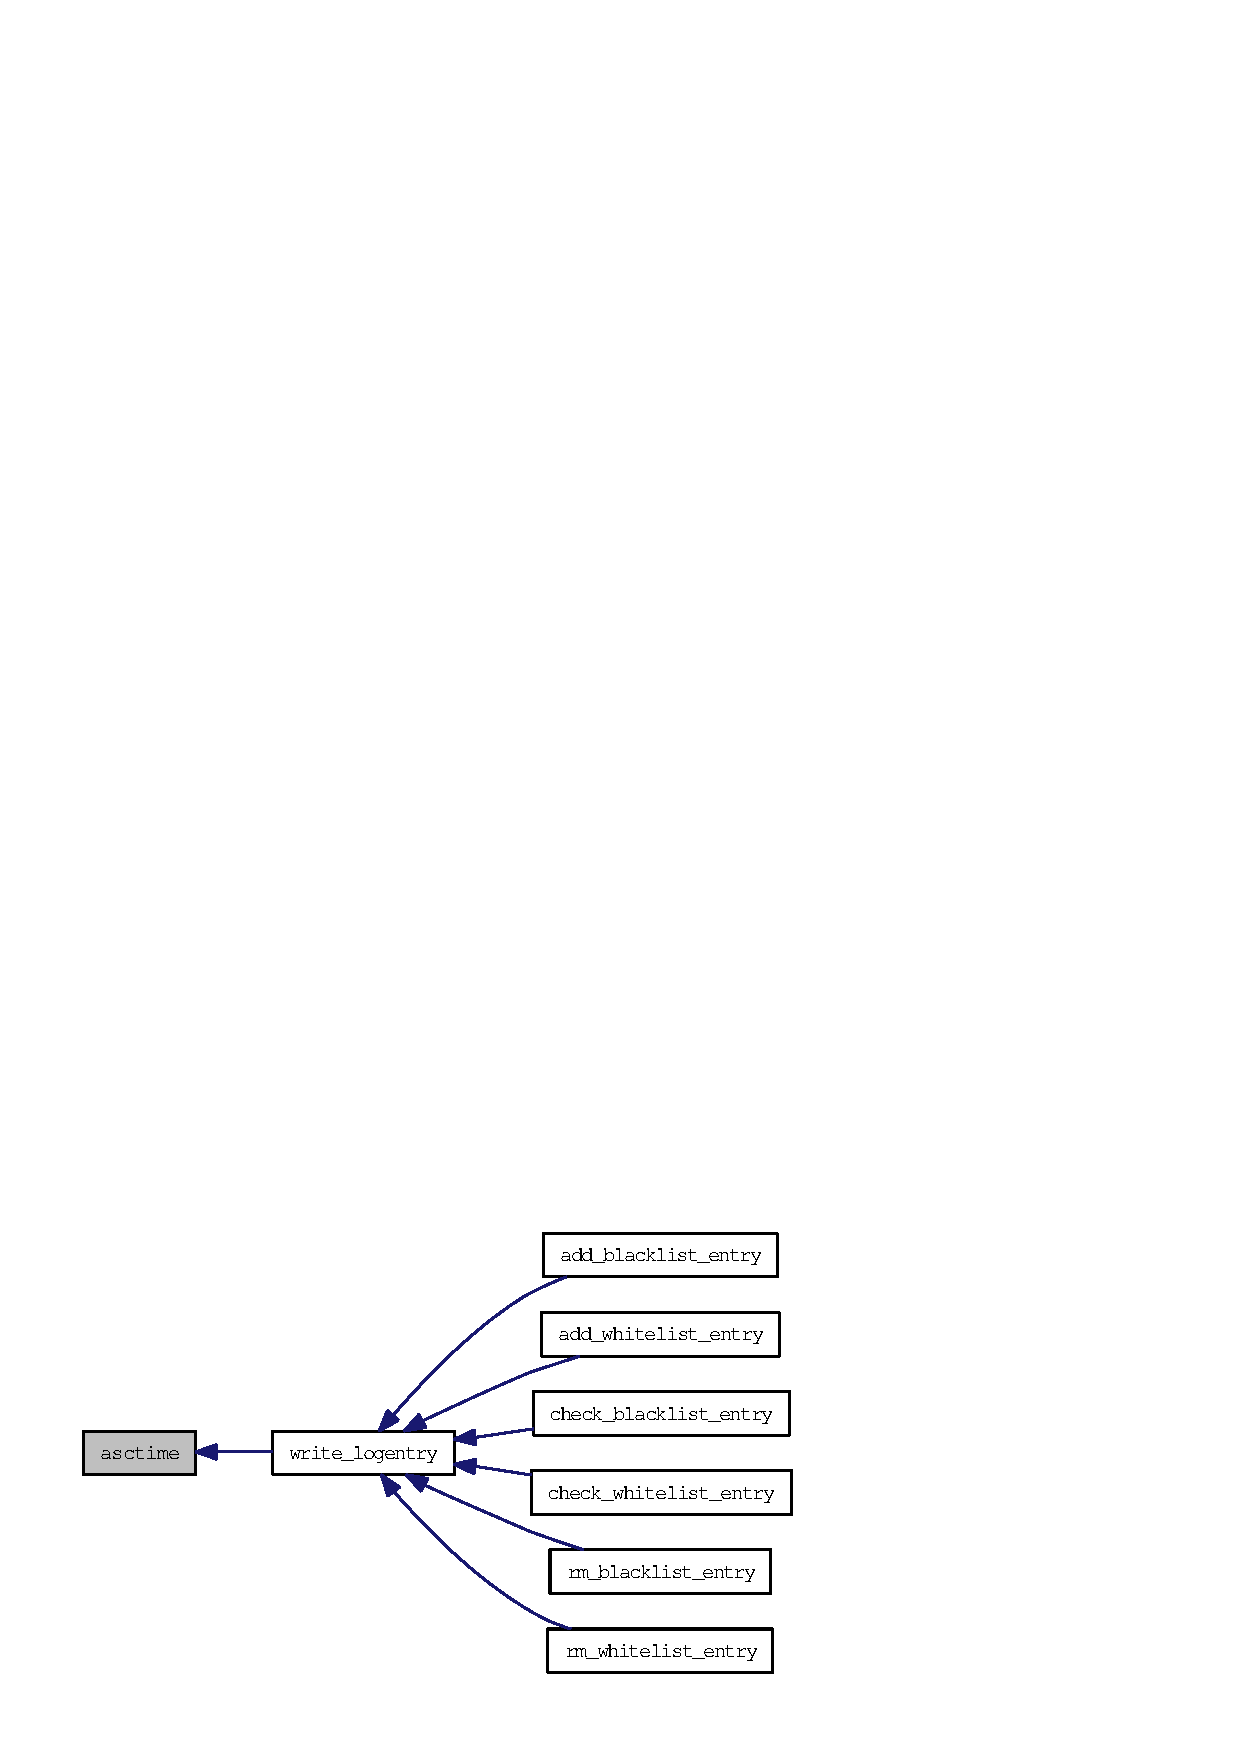
\includegraphics[width=348pt]{logfile_8c_68a0e9d22417dfcf9c0be64261352e64_icgraph}
\end{center}
\end{figure}
\hypertarget{logfile_8c_f71f5daf2025b4e30a18ccedf7c34863}{
\index{logfile.c@{logfile.c}!write\_\-logentry@{write\_\-logentry}}
\index{write\_\-logentry@{write\_\-logentry}!logfile.c@{logfile.c}}
\subsubsection{\setlength{\rightskip}{0pt plus 5cm}int write\_\-logentry (char $\ast$ {\em msg}, char $\ast$ {\em component}, int {\em flag})}}
\label{logfile_8c_f71f5daf2025b4e30a18ccedf7c34863}


Writes a logfile enty.

\begin{Desc}
\item[Parameters:]
\begin{description}
\item[{\em msg}]The message which should be written in the logfile. \item[{\em component}]The program which calls the write\_\-logentry function, for example \char`\"{}phonefirewall\char`\"{} \item[{\em flag}]What message should be written. Use the defined flags.\end{description}
\end{Desc}
\begin{Desc}
\item[Returns:]-1 if something fails, otherwise 0 \end{Desc}


Definition at line 56 of file logfile.c.

References asctime(), ERR\_\-FLAG, INFO\_\-FLAG, LOGFILE, MAX\_\-ENTRY\_\-LENGTH, UNKNOWN, and WARN\_\-FLAG.

Referenced by add\_\-entry(), check\_\-entry(), dbus\_\-listen(), get\_\-entry\_\-by\_\-name(), rm\_\-entry(), start\_\-daemon(), and stop\_\-daemon().

Here is the call graph for this function:\nopagebreak
\begin{figure}[H]
\begin{center}
\leavevmode
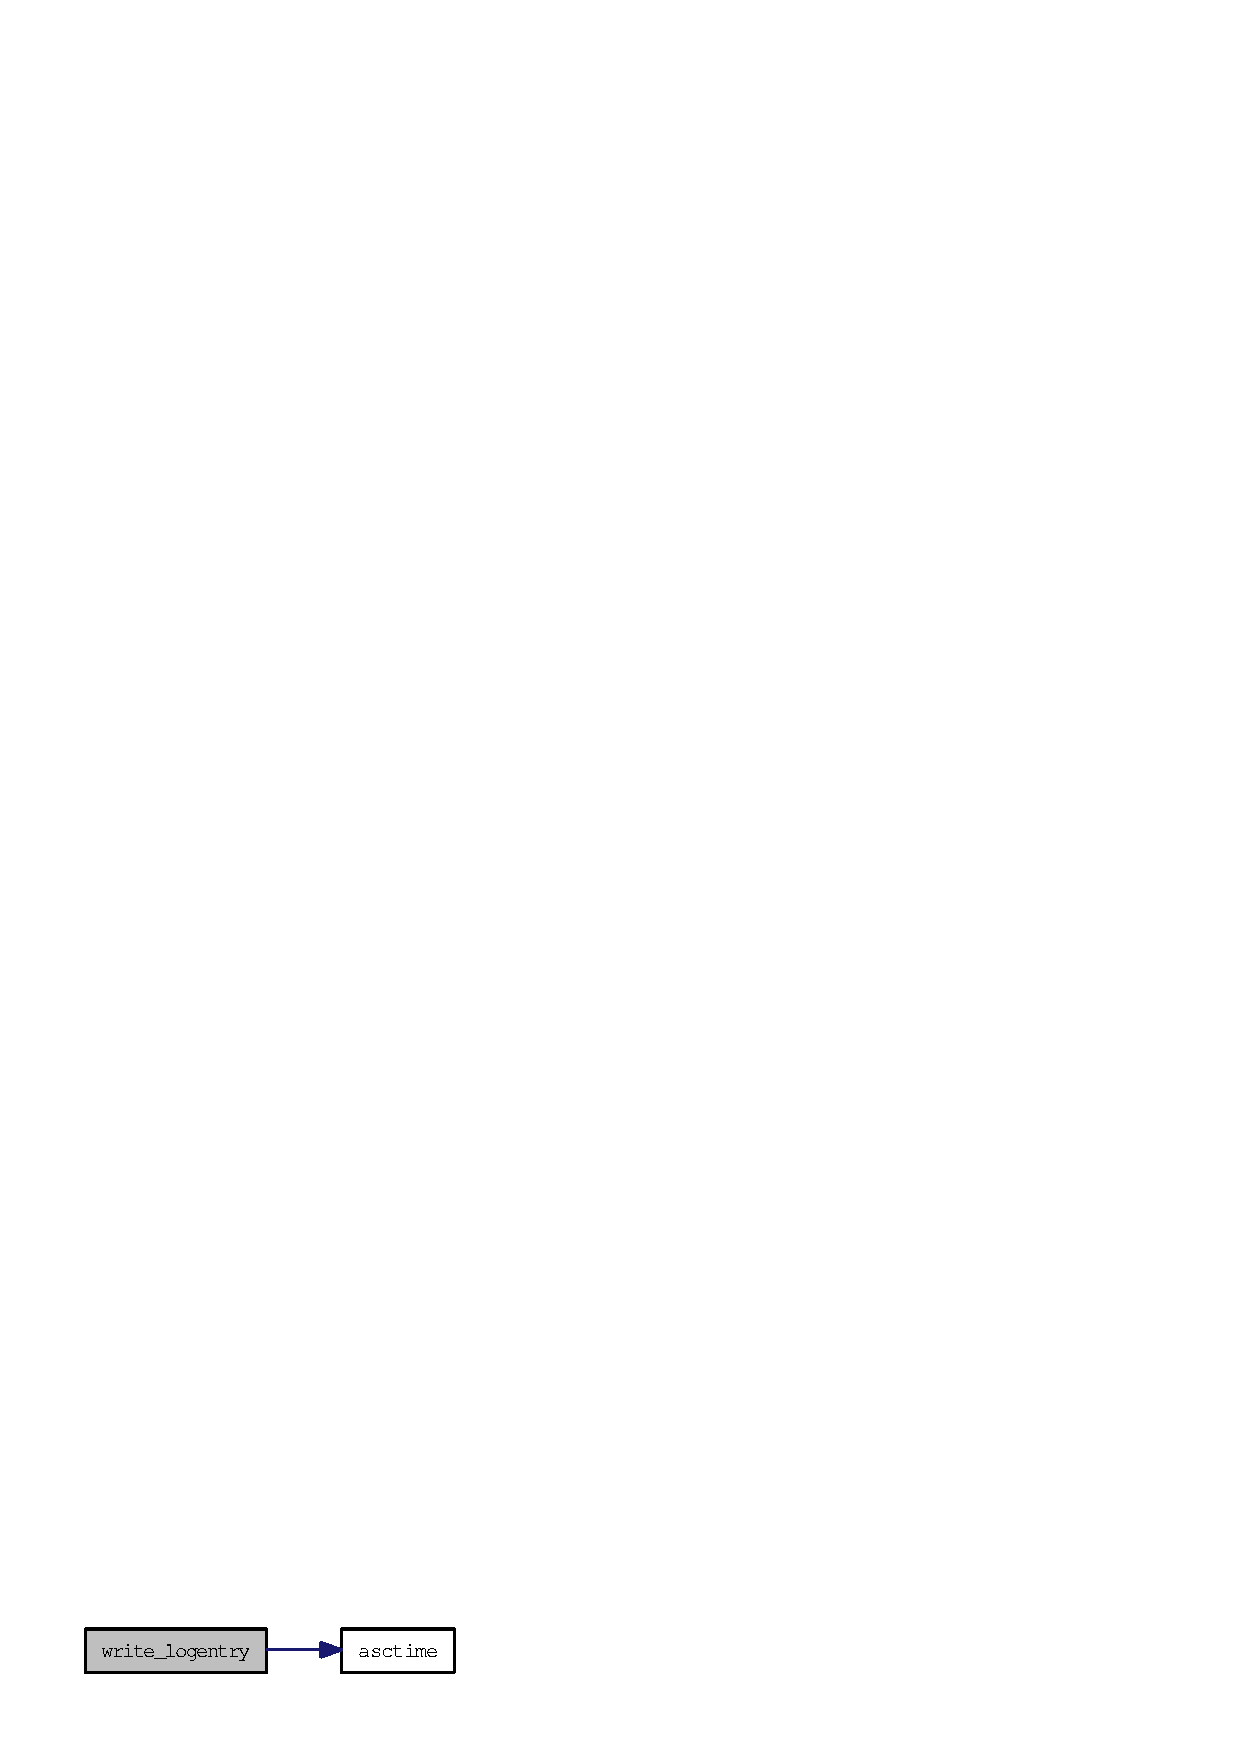
\includegraphics[width=111pt]{logfile_8c_f71f5daf2025b4e30a18ccedf7c34863_cgraph}
\end{center}
\end{figure}


Here is the caller graph for this function:\nopagebreak
\begin{figure}[H]
\begin{center}
\leavevmode
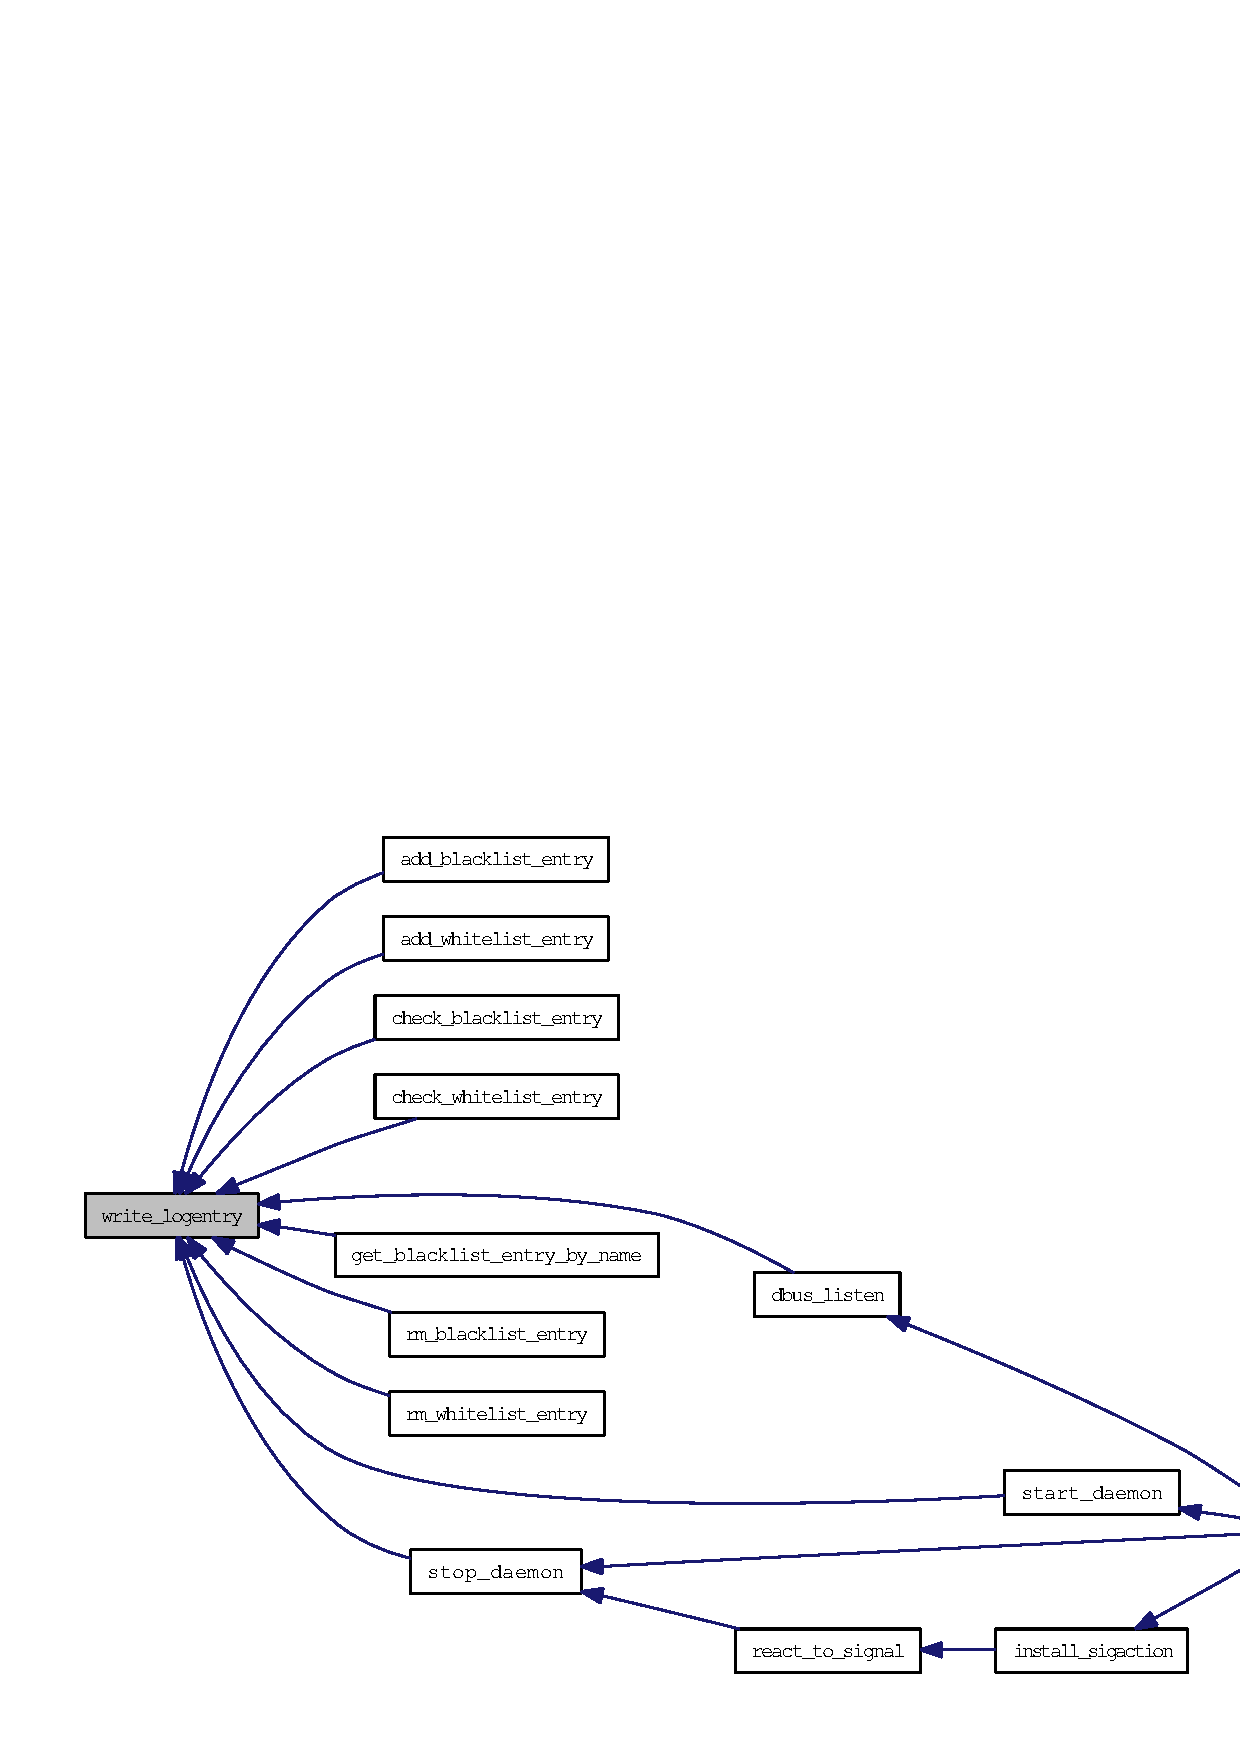
\includegraphics[width=303pt]{logfile_8c_f71f5daf2025b4e30a18ccedf7c34863_icgraph}
\end{center}
\end{figure}

\hypertarget{logfile_8h}{
\section{logfile.h File Reference}
\label{logfile_8h}\index{logfile.h@{logfile.h}}
}


This graph shows which files directly or indirectly include this file:\nopagebreak
\begin{figure}[H]
\begin{center}
\leavevmode
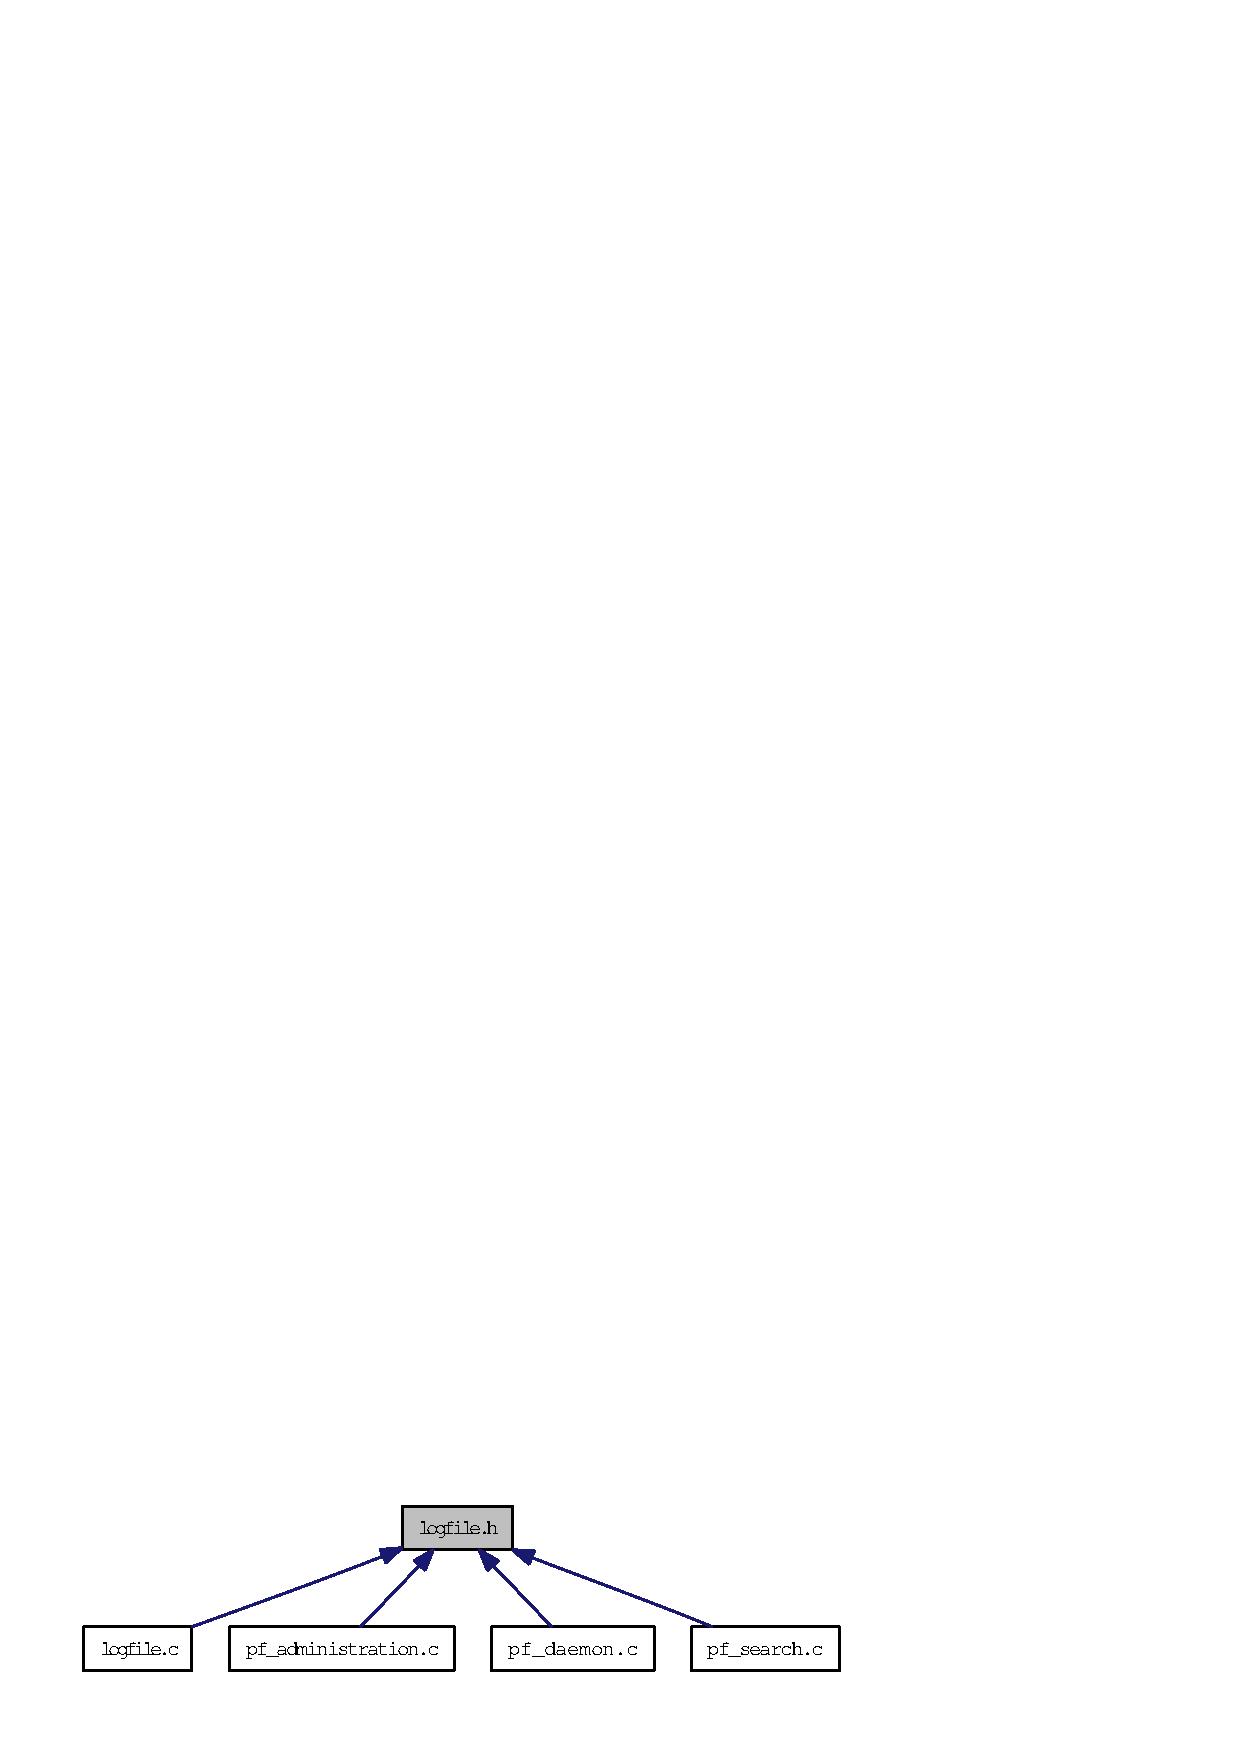
\includegraphics[width=256pt]{logfile_8h__dep__incl}
\end{center}
\end{figure}
\subsection*{Defines}
\begin{CompactItemize}
\item 
\#define \hyperlink{logfile_8h_6d3fef197146b932f5ad01fce683a66b}{LOGFILE}~\char`\"{}log/moksec.log\char`\"{}
\item 
\#define \hyperlink{logfile_8h_790d3f39336d5c73462ac5f113c79237}{MAX\_\-ENTRY\_\-LENGTH}~128
\item 
\#define \hyperlink{logfile_8h_c1ae4add974b9cfc6b5aaf8a578f01ab}{UNKNOWN}~0
\item 
\#define \hyperlink{logfile_8h_cd48c0293626a8577ef1c28ad58ca0d6}{ERR\_\-FLAG}~1
\item 
\#define \hyperlink{logfile_8h_d683e726fb2cb177c24b8cb84e80ea7d}{WARN\_\-FLAG}~2
\item 
\#define \hyperlink{logfile_8h_655cb5e43527221af659a76352b141ae}{INFO\_\-FLAG}~3
\end{CompactItemize}
\subsection*{Functions}
\begin{CompactItemize}
\item 
int \hyperlink{logfile_8h_f71f5daf2025b4e30a18ccedf7c34863}{write\_\-logentry} (char $\ast$msg, char $\ast$component, int flag)
\end{CompactItemize}


\subsection{Define Documentation}
\hypertarget{logfile_8h_cd48c0293626a8577ef1c28ad58ca0d6}{
\index{logfile.h@{logfile.h}!ERR\_\-FLAG@{ERR\_\-FLAG}}
\index{ERR\_\-FLAG@{ERR\_\-FLAG}!logfile.h@{logfile.h}}
\subsubsection{\setlength{\rightskip}{0pt plus 5cm}\#define ERR\_\-FLAG~1}}
\label{logfile_8h_cd48c0293626a8577ef1c28ad58ca0d6}




Definition at line 25 of file logfile.h.

Referenced by add\_\-blacklist\_\-entry(), add\_\-whitelist\_\-entry(), check\_\-blacklist\_\-entry(), check\_\-whitelist\_\-entry(), dbus\_\-listen(), get\_\-blacklist\_\-entry\_\-by\_\-name(), rm\_\-blacklist\_\-entry(), rm\_\-whitelist\_\-entry(), and write\_\-logentry().\hypertarget{logfile_8h_655cb5e43527221af659a76352b141ae}{
\index{logfile.h@{logfile.h}!INFO\_\-FLAG@{INFO\_\-FLAG}}
\index{INFO\_\-FLAG@{INFO\_\-FLAG}!logfile.h@{logfile.h}}
\subsubsection{\setlength{\rightskip}{0pt plus 5cm}\#define INFO\_\-FLAG~3}}
\label{logfile_8h_655cb5e43527221af659a76352b141ae}




Definition at line 27 of file logfile.h.

Referenced by check\_\-blacklist\_\-entry(), check\_\-whitelist\_\-entry(), dbus\_\-listen(), start\_\-daemon(), stop\_\-daemon(), and write\_\-logentry().\hypertarget{logfile_8h_6d3fef197146b932f5ad01fce683a66b}{
\index{logfile.h@{logfile.h}!LOGFILE@{LOGFILE}}
\index{LOGFILE@{LOGFILE}!logfile.h@{logfile.h}}
\subsubsection{\setlength{\rightskip}{0pt plus 5cm}\#define LOGFILE~\char`\"{}log/moksec.log\char`\"{}}}
\label{logfile_8h_6d3fef197146b932f5ad01fce683a66b}




Definition at line 21 of file logfile.h.

Referenced by write\_\-logentry().\hypertarget{logfile_8h_790d3f39336d5c73462ac5f113c79237}{
\index{logfile.h@{logfile.h}!MAX\_\-ENTRY\_\-LENGTH@{MAX\_\-ENTRY\_\-LENGTH}}
\index{MAX\_\-ENTRY\_\-LENGTH@{MAX\_\-ENTRY\_\-LENGTH}!logfile.h@{logfile.h}}
\subsubsection{\setlength{\rightskip}{0pt plus 5cm}\#define MAX\_\-ENTRY\_\-LENGTH~128}}
\label{logfile_8h_790d3f39336d5c73462ac5f113c79237}




Definition at line 22 of file logfile.h.

Referenced by write\_\-logentry().\hypertarget{logfile_8h_c1ae4add974b9cfc6b5aaf8a578f01ab}{
\index{logfile.h@{logfile.h}!UNKNOWN@{UNKNOWN}}
\index{UNKNOWN@{UNKNOWN}!logfile.h@{logfile.h}}
\subsubsection{\setlength{\rightskip}{0pt plus 5cm}\#define UNKNOWN~0}}
\label{logfile_8h_c1ae4add974b9cfc6b5aaf8a578f01ab}




Definition at line 24 of file logfile.h.

Referenced by write\_\-logentry().\hypertarget{logfile_8h_d683e726fb2cb177c24b8cb84e80ea7d}{
\index{logfile.h@{logfile.h}!WARN\_\-FLAG@{WARN\_\-FLAG}}
\index{WARN\_\-FLAG@{WARN\_\-FLAG}!logfile.h@{logfile.h}}
\subsubsection{\setlength{\rightskip}{0pt plus 5cm}\#define WARN\_\-FLAG~2}}
\label{logfile_8h_d683e726fb2cb177c24b8cb84e80ea7d}




Definition at line 26 of file logfile.h.

Referenced by write\_\-logentry().

\subsection{Function Documentation}
\hypertarget{logfile_8h_f71f5daf2025b4e30a18ccedf7c34863}{
\index{logfile.h@{logfile.h}!write\_\-logentry@{write\_\-logentry}}
\index{write\_\-logentry@{write\_\-logentry}!logfile.h@{logfile.h}}
\subsubsection{\setlength{\rightskip}{0pt plus 5cm}int write\_\-logentry (char $\ast$ {\em msg}, char $\ast$ {\em component}, int {\em flag})}}
\label{logfile_8h_f71f5daf2025b4e30a18ccedf7c34863}


Writes a logfile enty.

\begin{Desc}
\item[Parameters:]
\begin{description}
\item[{\em msg}]The message which should be written in the logfile. \item[{\em component}]The program which calls the write\_\-logentry function, for example \char`\"{}phonefirewall\char`\"{} \item[{\em flag}]What message should be written. Use the defined flags.\end{description}
\end{Desc}
\begin{Desc}
\item[Returns:]-1 if something fails, otherwise 0 \end{Desc}


Definition at line 56 of file logfile.c.

References asctime(), ERR\_\-FLAG, INFO\_\-FLAG, LOGFILE, MAX\_\-ENTRY\_\-LENGTH, UNKNOWN, and WARN\_\-FLAG.

Referenced by add\_\-blacklist\_\-entry(), add\_\-whitelist\_\-entry(), check\_\-blacklist\_\-entry(), check\_\-whitelist\_\-entry(), dbus\_\-listen(), get\_\-blacklist\_\-entry\_\-by\_\-name(), rm\_\-blacklist\_\-entry(), rm\_\-whitelist\_\-entry(), start\_\-daemon(), and stop\_\-daemon().

Here is the call graph for this function:\nopagebreak
\begin{figure}[H]
\begin{center}
\leavevmode
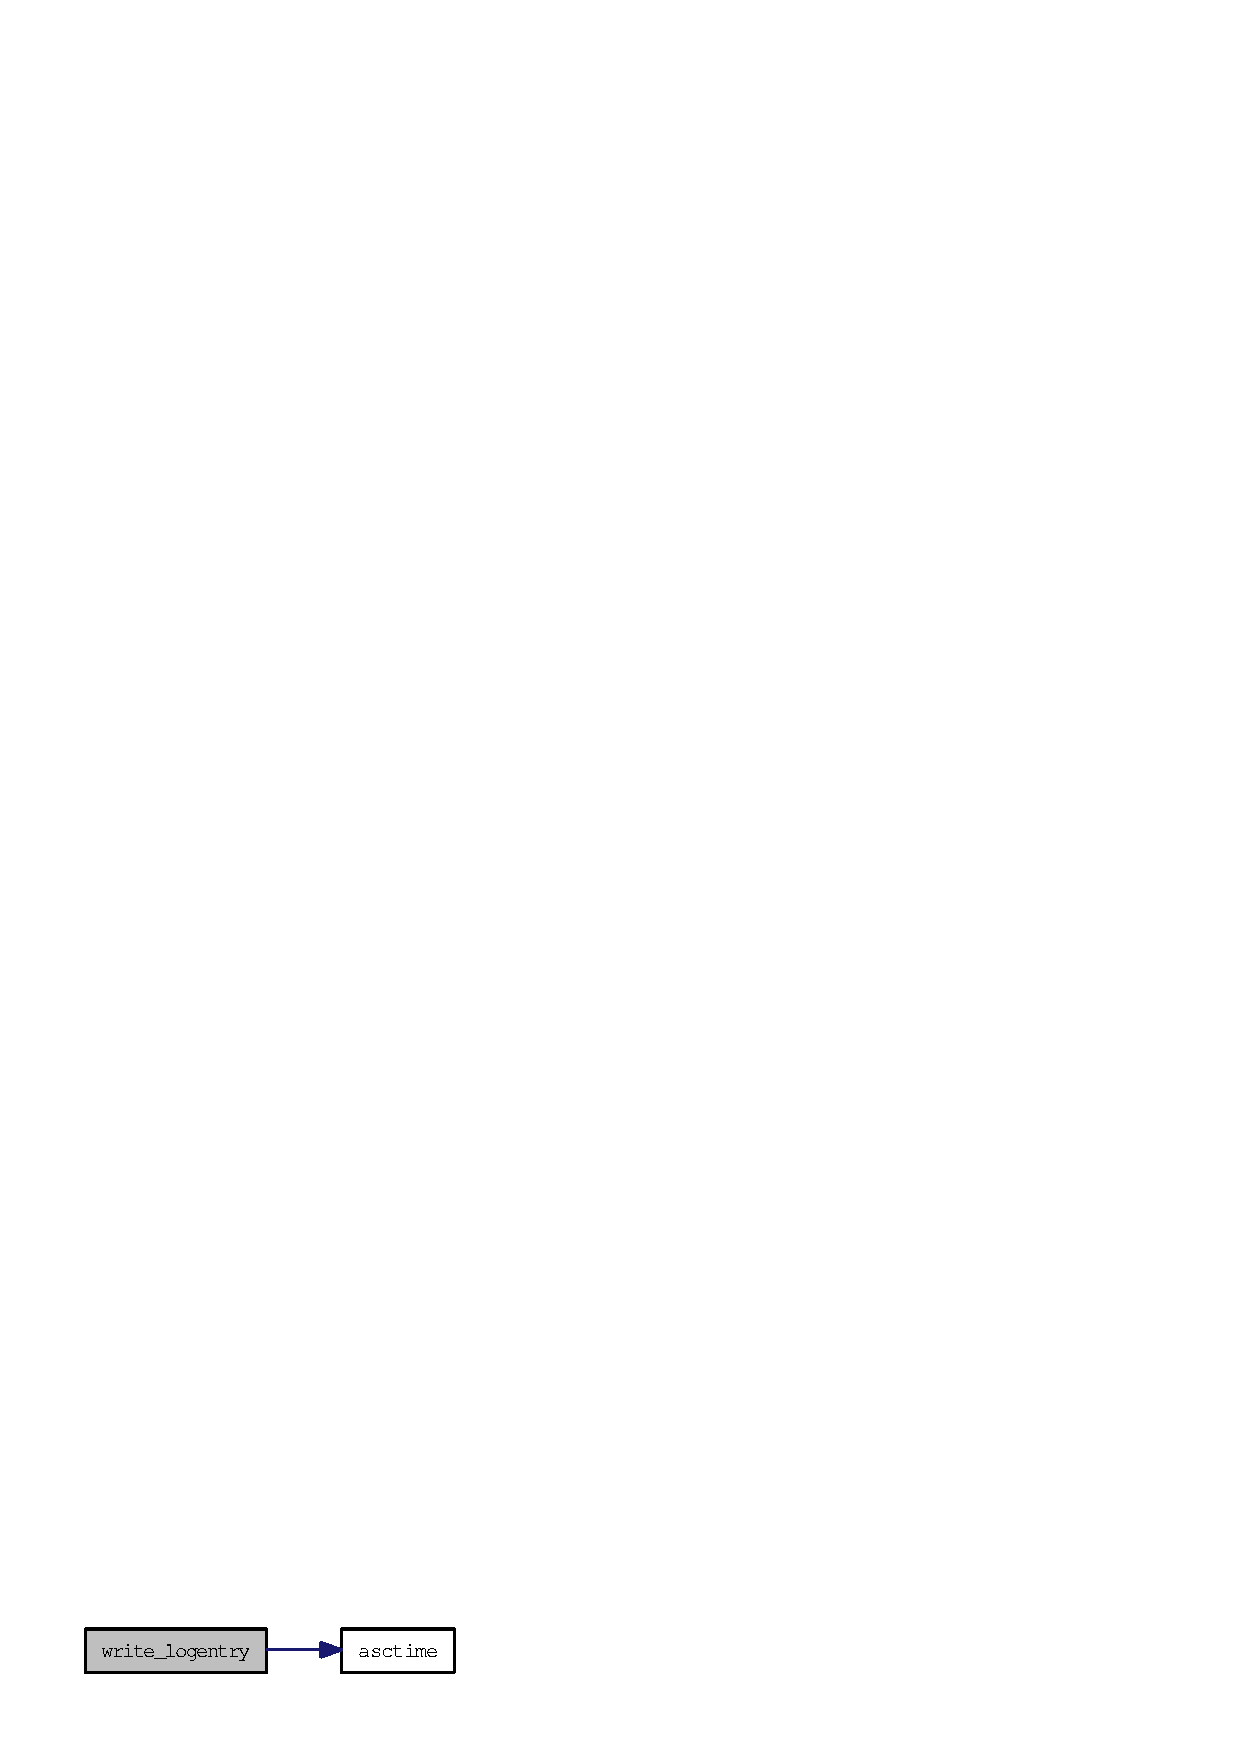
\includegraphics[width=111pt]{logfile_8h_f71f5daf2025b4e30a18ccedf7c34863_cgraph}
\end{center}
\end{figure}


Here is the caller graph for this function:\nopagebreak
\begin{figure}[H]
\begin{center}
\leavevmode
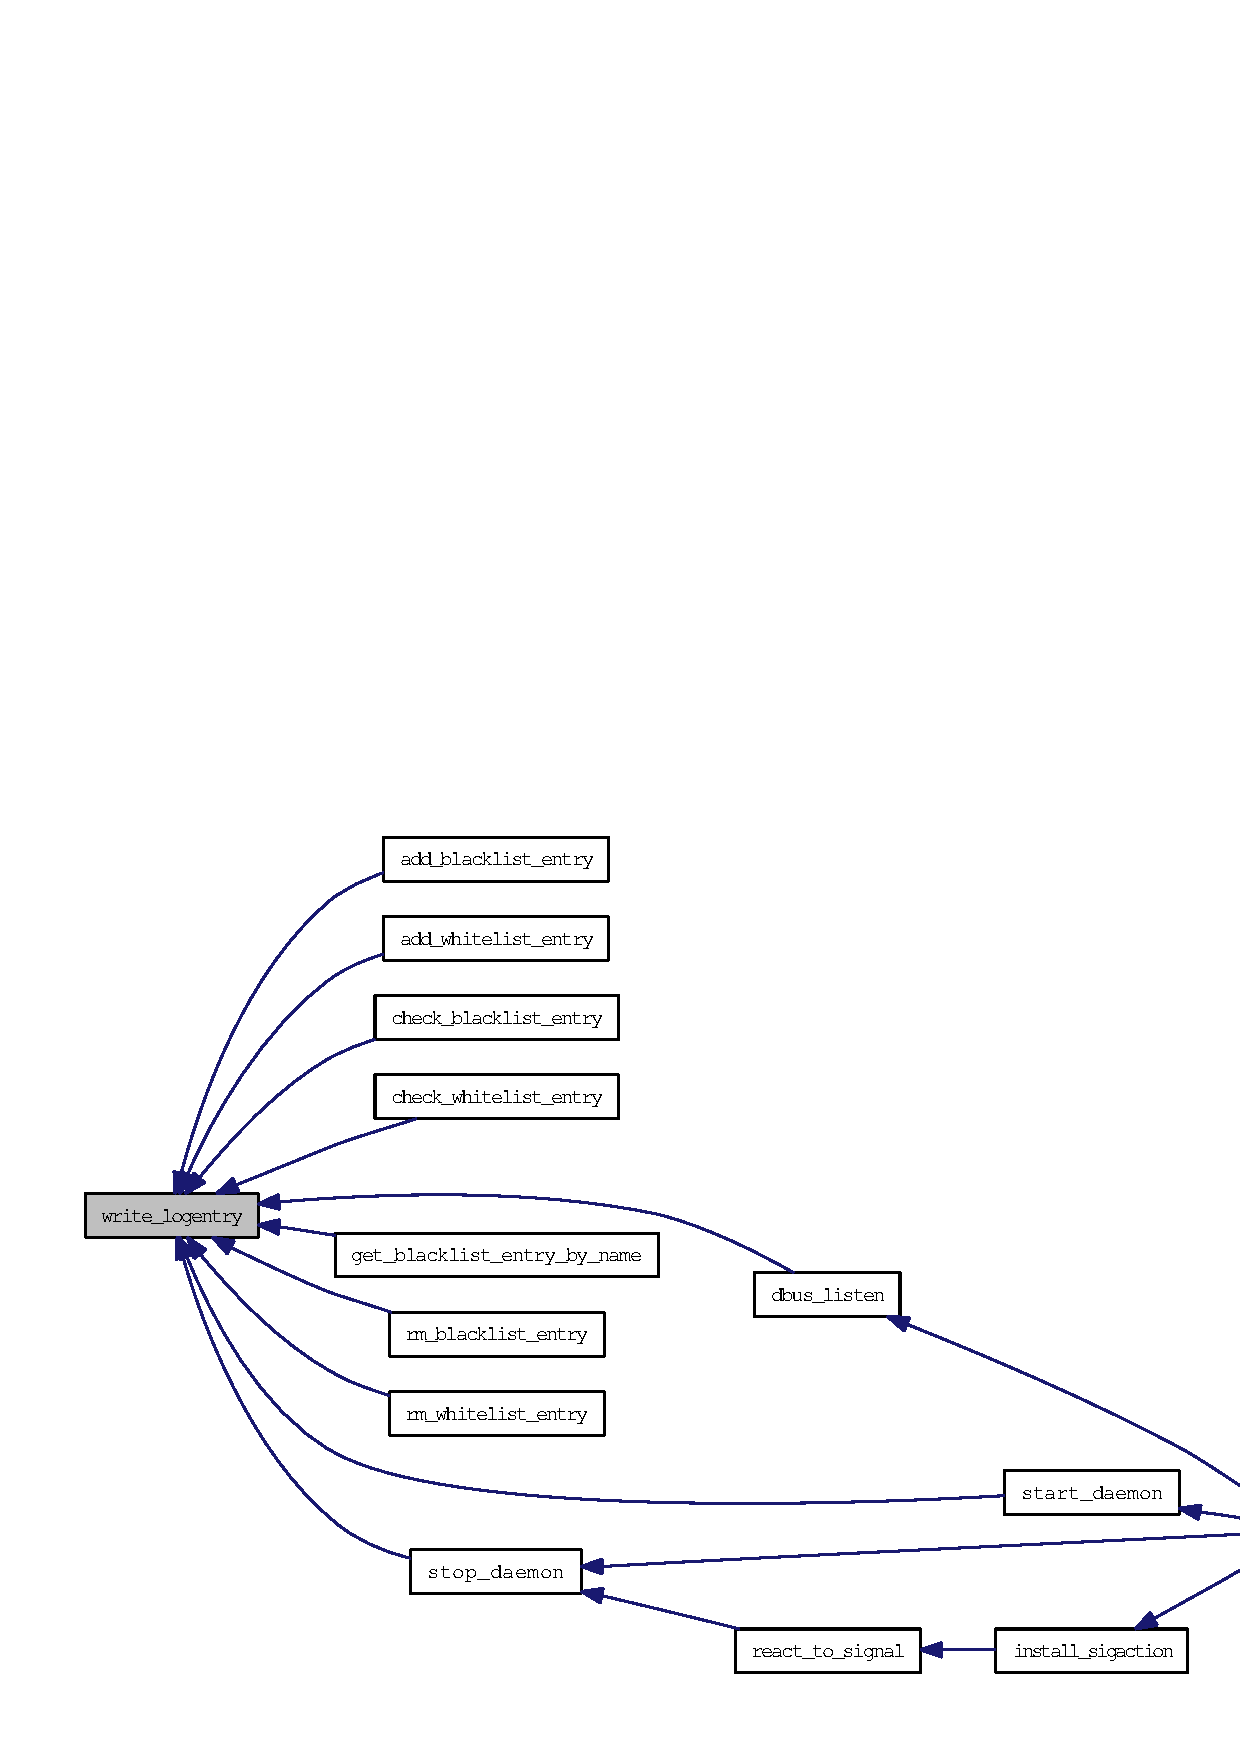
\includegraphics[width=325pt]{logfile_8h_f71f5daf2025b4e30a18ccedf7c34863_icgraph}
\end{center}
\end{figure}

\hypertarget{pf__daemon_8c}{
\section{pf\_\-daemon.c File Reference}
\label{pf__daemon_8c}\index{pf\_\-daemon.c@{pf\_\-daemon.c}}
}
{\tt \#include $<$stdio.h$>$}\par
{\tt \#include $<$stdlib.h$>$}\par
{\tt \#include $<$unistd.h$>$}\par
{\tt \#include $<$errno.h$>$}\par
{\tt \#include $<$stdbool.h$>$}\par
{\tt \#include $<$dbus/dbus.h$>$}\par
{\tt \#include \char`\"{}libphonefirewall.h\char`\"{}}\par


Include dependency graph for pf\_\-daemon.c:\nopagebreak
\begin{figure}[H]
\begin{center}
\leavevmode
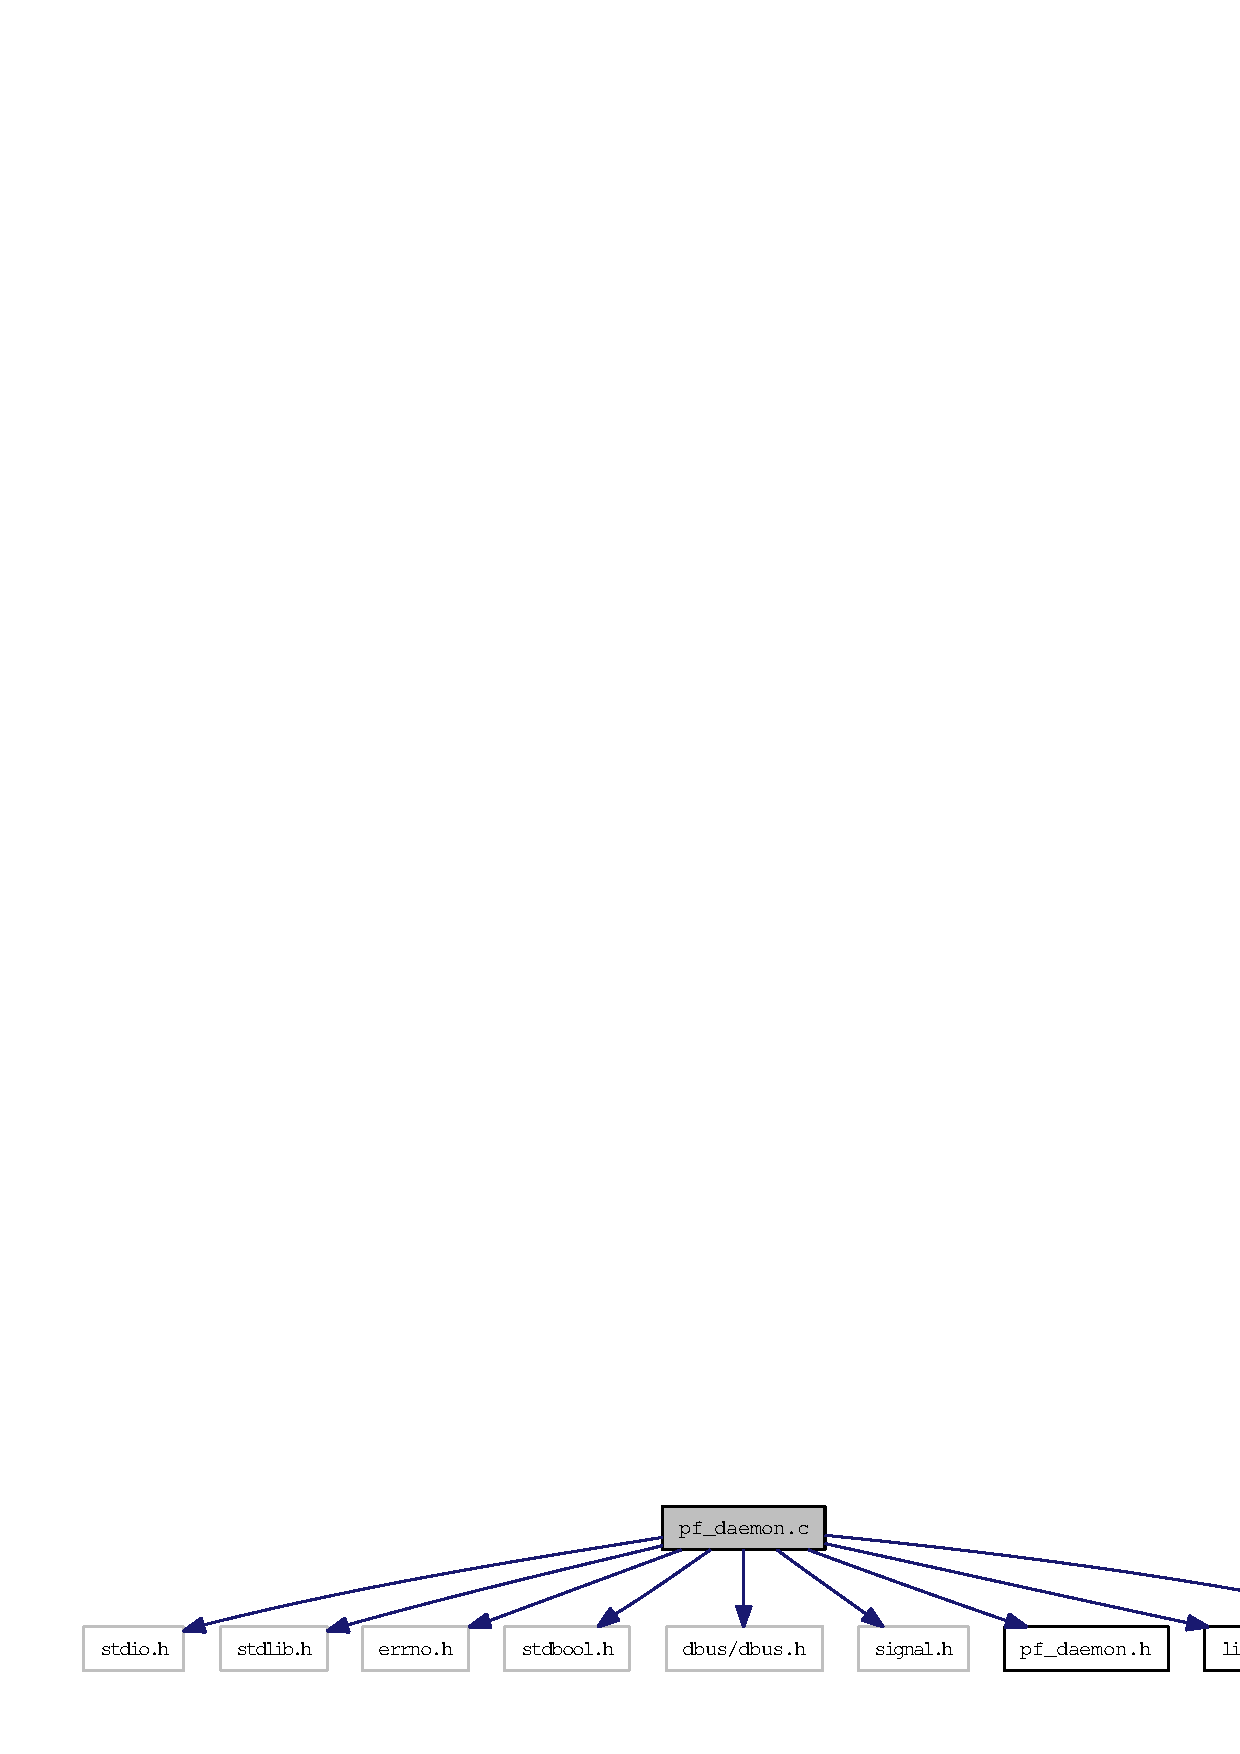
\includegraphics[width=299pt]{pf__daemon_8c__incl}
\end{center}
\end{figure}
\subsection*{Defines}
\begin{CompactItemize}
\item 
\#define \hyperlink{pf__daemon_8c_551ae9e7796a78ff54bc98eef4e74498}{LOCKFILE}~\char`\"{}.lock\char`\"{}
\end{CompactItemize}
\subsection*{Functions}
\begin{CompactItemize}
\item 
void \hyperlink{pf__daemon_8c_0e2f72a981c64aefe314e745b28b6387}{start\_\-daemon} ()
\item 
void \hyperlink{pf__daemon_8c_725630dc6f9856b1349100761924050f}{stop\_\-daemon} ()
\item 
void \hyperlink{pf__daemon_8c_db0a9558ddd4dc0bbad7b5ddfc5231c6}{dbus\_\-listen} ()
\item 
int \hyperlink{pf__daemon_8c_3c04138a5bfe5d72780bb7e82a18e627}{main} (int argc, char $\ast$$\ast$argv)
\end{CompactItemize}


\subsection{Define Documentation}
\hypertarget{pf__daemon_8c_551ae9e7796a78ff54bc98eef4e74498}{
\index{pf\_\-daemon.c@{pf\_\-daemon.c}!LOCKFILE@{LOCKFILE}}
\index{LOCKFILE@{LOCKFILE}!pf_daemon.c@{pf\_\-daemon.c}}
\subsubsection{\setlength{\rightskip}{0pt plus 5cm}\#define LOCKFILE~\char`\"{}.lock\char`\"{}}}
\label{pf__daemon_8c_551ae9e7796a78ff54bc98eef4e74498}




Definition at line 9 of file pf\_\-daemon.c.

Referenced by start\_\-daemon(), and stop\_\-daemon().

\subsection{Function Documentation}
\hypertarget{pf__daemon_8c_db0a9558ddd4dc0bbad7b5ddfc5231c6}{
\index{pf\_\-daemon.c@{pf\_\-daemon.c}!dbus\_\-listen@{dbus\_\-listen}}
\index{dbus\_\-listen@{dbus\_\-listen}!pf_daemon.c@{pf\_\-daemon.c}}
\subsubsection{\setlength{\rightskip}{0pt plus 5cm}void dbus\_\-listen ()}}
\label{pf__daemon_8c_db0a9558ddd4dc0bbad7b5ddfc5231c6}


Function that provides method calls.

Bus name: to.networld.moksec.phonefirewall Object name: to.networld.moksec.phonefirewall.Object interface: to.networld.moksec.phonefirewall.Checking methods: checkblacklist(...) checkwhitelist(...) 

Definition at line 75 of file pf\_\-daemon.c.

Referenced by main().

Here is the caller graph for this function:\nopagebreak
\begin{figure}[H]
\begin{center}
\leavevmode
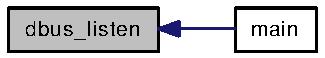
\includegraphics[width=96pt]{pf__daemon_8c_db0a9558ddd4dc0bbad7b5ddfc5231c6_icgraph}
\end{center}
\end{figure}
\hypertarget{pf__daemon_8c_3c04138a5bfe5d72780bb7e82a18e627}{
\index{pf\_\-daemon.c@{pf\_\-daemon.c}!main@{main}}
\index{main@{main}!pf_daemon.c@{pf\_\-daemon.c}}
\subsubsection{\setlength{\rightskip}{0pt plus 5cm}int main (int {\em argc}, char $\ast$$\ast$ {\em argv})}}
\label{pf__daemon_8c_3c04138a5bfe5d72780bb7e82a18e627}




Definition at line 34 of file pf\_\-daemon.c.

References dbus\_\-listen(), start\_\-daemon(), and stop\_\-daemon().

Here is the call graph for this function:\nopagebreak
\begin{figure}[H]
\begin{center}
\leavevmode
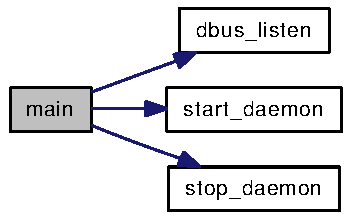
\includegraphics[width=102pt]{pf__daemon_8c_3c04138a5bfe5d72780bb7e82a18e627_cgraph}
\end{center}
\end{figure}
\hypertarget{pf__daemon_8c_0e2f72a981c64aefe314e745b28b6387}{
\index{pf\_\-daemon.c@{pf\_\-daemon.c}!start\_\-daemon@{start\_\-daemon}}
\index{start\_\-daemon@{start\_\-daemon}!pf_daemon.c@{pf\_\-daemon.c}}
\subsubsection{\setlength{\rightskip}{0pt plus 5cm}void start\_\-daemon ()}}
\label{pf__daemon_8c_0e2f72a981c64aefe314e745b28b6387}


Starts the program as a daemon and creates a lockfile (specified in the LOCKFILE constant). So it's impossible to start the daemon twice. 

Definition at line 45 of file pf\_\-daemon.c.

References LOCKFILE.

Referenced by main().

Here is the caller graph for this function:\nopagebreak
\begin{figure}[H]
\begin{center}
\leavevmode
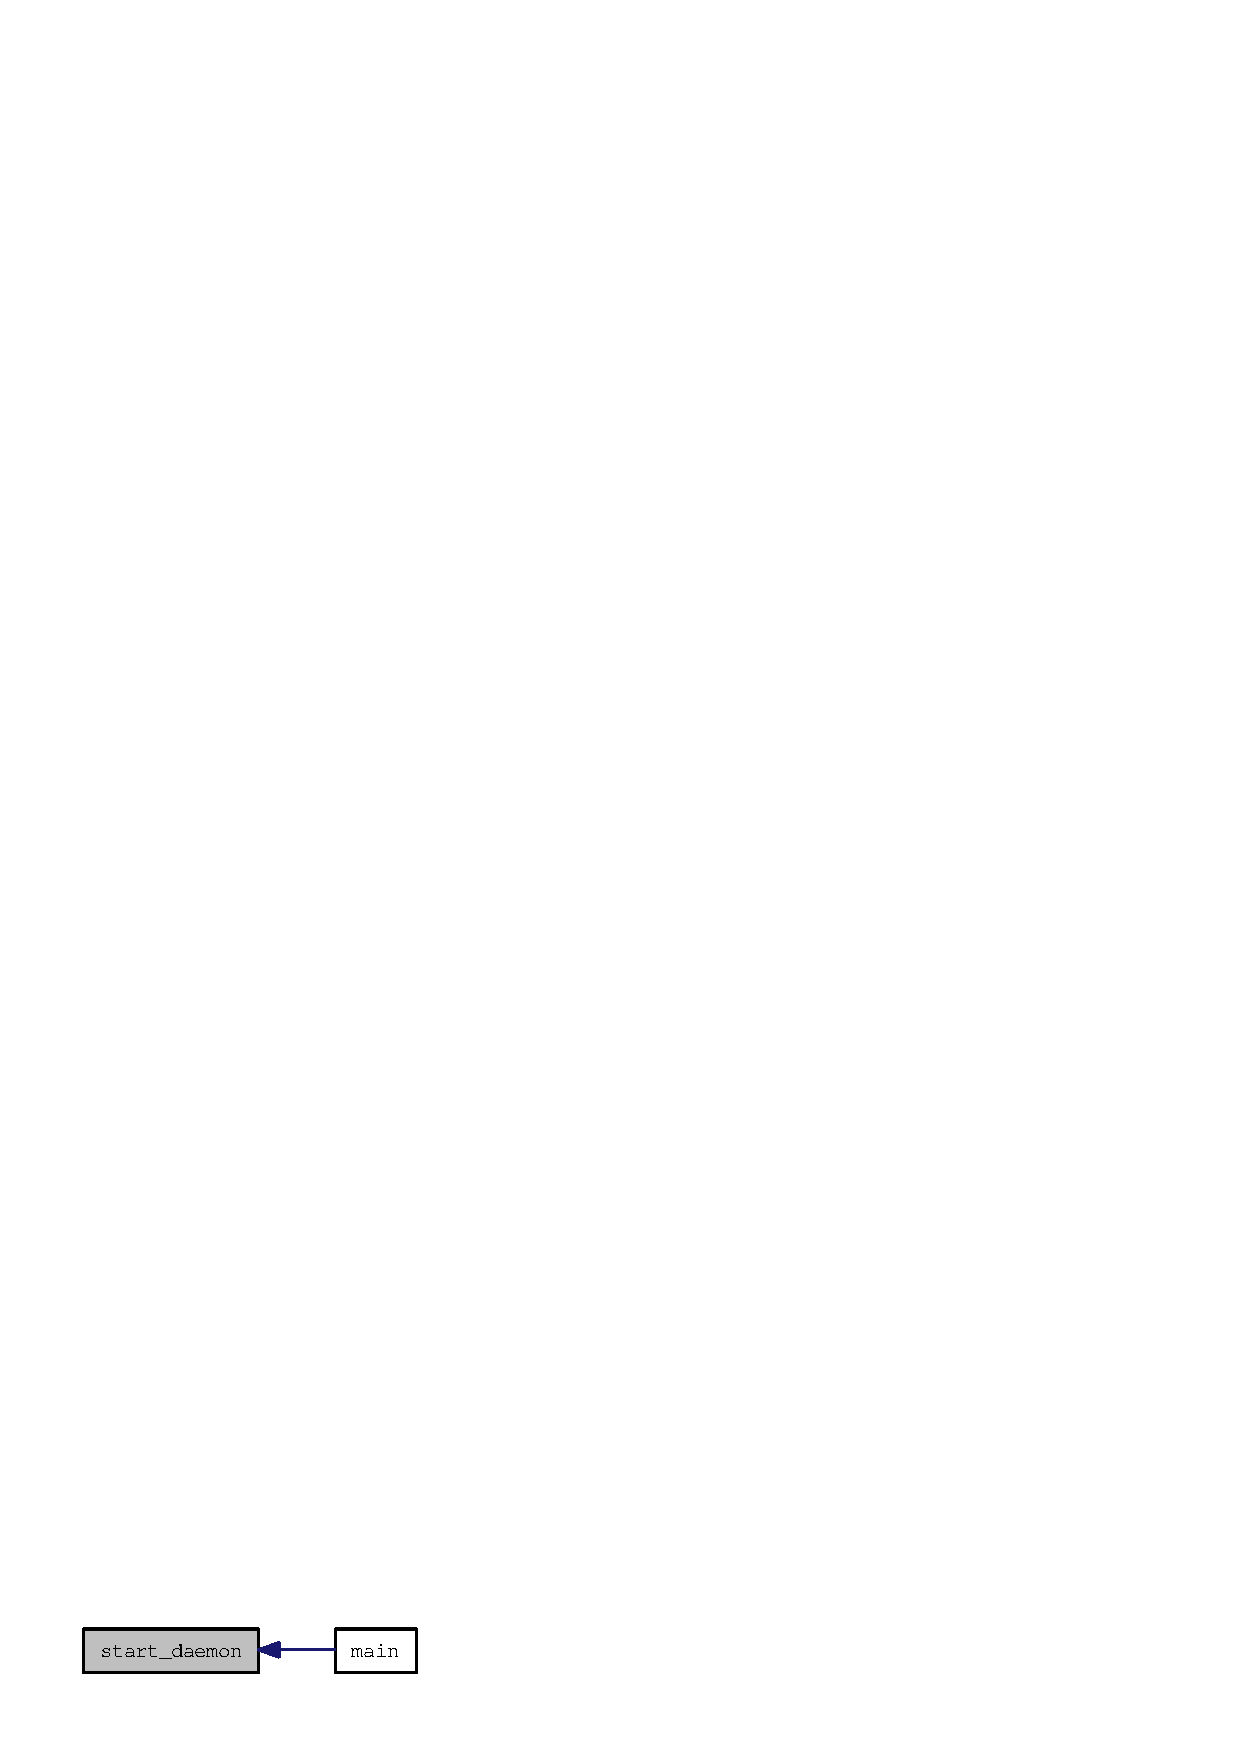
\includegraphics[width=102pt]{pf__daemon_8c_0e2f72a981c64aefe314e745b28b6387_icgraph}
\end{center}
\end{figure}
\hypertarget{pf__daemon_8c_725630dc6f9856b1349100761924050f}{
\index{pf\_\-daemon.c@{pf\_\-daemon.c}!stop\_\-daemon@{stop\_\-daemon}}
\index{stop\_\-daemon@{stop\_\-daemon}!pf_daemon.c@{pf\_\-daemon.c}}
\subsubsection{\setlength{\rightskip}{0pt plus 5cm}void stop\_\-daemon ()}}
\label{pf__daemon_8c_725630dc6f9856b1349100761924050f}


Stops the daemon and deletes the lockfile, so a new instance can be started. 

Definition at line 69 of file pf\_\-daemon.c.

References LOCKFILE.

Referenced by main().

Here is the caller graph for this function:\nopagebreak
\begin{figure}[H]
\begin{center}
\leavevmode
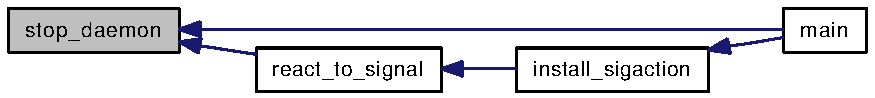
\includegraphics[width=101pt]{pf__daemon_8c_725630dc6f9856b1349100761924050f_icgraph}
\end{center}
\end{figure}

\hypertarget{pf__daemon_8h}{
\section{pf\_\-daemon.h File Reference}
\label{pf__daemon_8h}\index{pf\_\-daemon.h@{pf\_\-daemon.h}}
}


This graph shows which files directly or indirectly include this file:\nopagebreak
\begin{figure}[H]
\begin{center}
\leavevmode
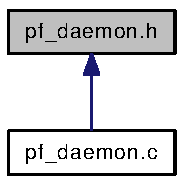
\includegraphics[width=62pt]{pf__daemon_8h__dep__incl}
\end{center}
\end{figure}
\subsection*{Defines}
\begin{CompactItemize}
\item 
\#define \hyperlink{pf__daemon_8h_551ae9e7796a78ff54bc98eef4e74498}{LOCKFILE}~\char`\"{}.lock\char`\"{}
\end{CompactItemize}
\subsection*{Functions}
\begin{CompactItemize}
\item 
void \hyperlink{pf__daemon_8h_0e2f72a981c64aefe314e745b28b6387}{start\_\-daemon} ()
\item 
void \hyperlink{pf__daemon_8h_725630dc6f9856b1349100761924050f}{stop\_\-daemon} ()
\item 
void \hyperlink{pf__daemon_8h_db0a9558ddd4dc0bbad7b5ddfc5231c6}{dbus\_\-listen} ()
\end{CompactItemize}


\subsection{Define Documentation}
\hypertarget{pf__daemon_8h_551ae9e7796a78ff54bc98eef4e74498}{
\index{pf\_\-daemon.h@{pf\_\-daemon.h}!LOCKFILE@{LOCKFILE}}
\index{LOCKFILE@{LOCKFILE}!pf_daemon.h@{pf\_\-daemon.h}}
\subsubsection{\setlength{\rightskip}{0pt plus 5cm}\#define LOCKFILE~\char`\"{}.lock\char`\"{}}}
\label{pf__daemon_8h_551ae9e7796a78ff54bc98eef4e74498}




Definition at line 21 of file pf\_\-daemon.h.

Referenced by start\_\-daemon(), and stop\_\-daemon().

\subsection{Function Documentation}
\hypertarget{pf__daemon_8h_db0a9558ddd4dc0bbad7b5ddfc5231c6}{
\index{pf\_\-daemon.h@{pf\_\-daemon.h}!dbus\_\-listen@{dbus\_\-listen}}
\index{dbus\_\-listen@{dbus\_\-listen}!pf_daemon.h@{pf\_\-daemon.h}}
\subsubsection{\setlength{\rightskip}{0pt plus 5cm}void dbus\_\-listen ()}}
\label{pf__daemon_8h_db0a9558ddd4dc0bbad7b5ddfc5231c6}


Function that provides method calls.

Bus name: to.networld.moksec.phonefirewall Object name: to.networld.moksec.phonefirewall.Object interface: to.networld.moksec.phonefirewall.Checking methods: checkblacklist(...) checkwhitelist(...) \hypertarget{pf__daemon_8h_0e2f72a981c64aefe314e745b28b6387}{
\index{pf\_\-daemon.h@{pf\_\-daemon.h}!start\_\-daemon@{start\_\-daemon}}
\index{start\_\-daemon@{start\_\-daemon}!pf_daemon.h@{pf\_\-daemon.h}}
\subsubsection{\setlength{\rightskip}{0pt plus 5cm}void start\_\-daemon ()}}
\label{pf__daemon_8h_0e2f72a981c64aefe314e745b28b6387}


Starts the program as a daemon and creates a lockfile (specified in the LOCKFILE constant). So it's impossible to start the daemon twice. \hypertarget{pf__daemon_8h_725630dc6f9856b1349100761924050f}{
\index{pf\_\-daemon.h@{pf\_\-daemon.h}!stop\_\-daemon@{stop\_\-daemon}}
\index{stop\_\-daemon@{stop\_\-daemon}!pf_daemon.h@{pf\_\-daemon.h}}
\subsubsection{\setlength{\rightskip}{0pt plus 5cm}void stop\_\-daemon ()}}
\label{pf__daemon_8h_725630dc6f9856b1349100761924050f}


Stops the daemon and deletes the lockfile, so a new instance can be started. 
\hypertarget{phonefirewall__administration_8c}{
\section{phonefirewall\_\-administration.c File Reference}
\label{phonefirewall__administration_8c}\index{phonefirewall\_\-administration.c@{phonefirewall\_\-administration.c}}
}
{\tt \#include $<$stdio.h$>$}\par
{\tt \#include $<$stdlib.h$>$}\par
{\tt \#include $<$errno.h$>$}\par
{\tt \#include $<$string.h$>$}\par
{\tt \#include \char`\"{}libphonefirewall.h\char`\"{}}\par


Include dependency graph for phonefirewall\_\-administration.c:\nopagebreak
\begin{figure}[H]
\begin{center}
\leavevmode
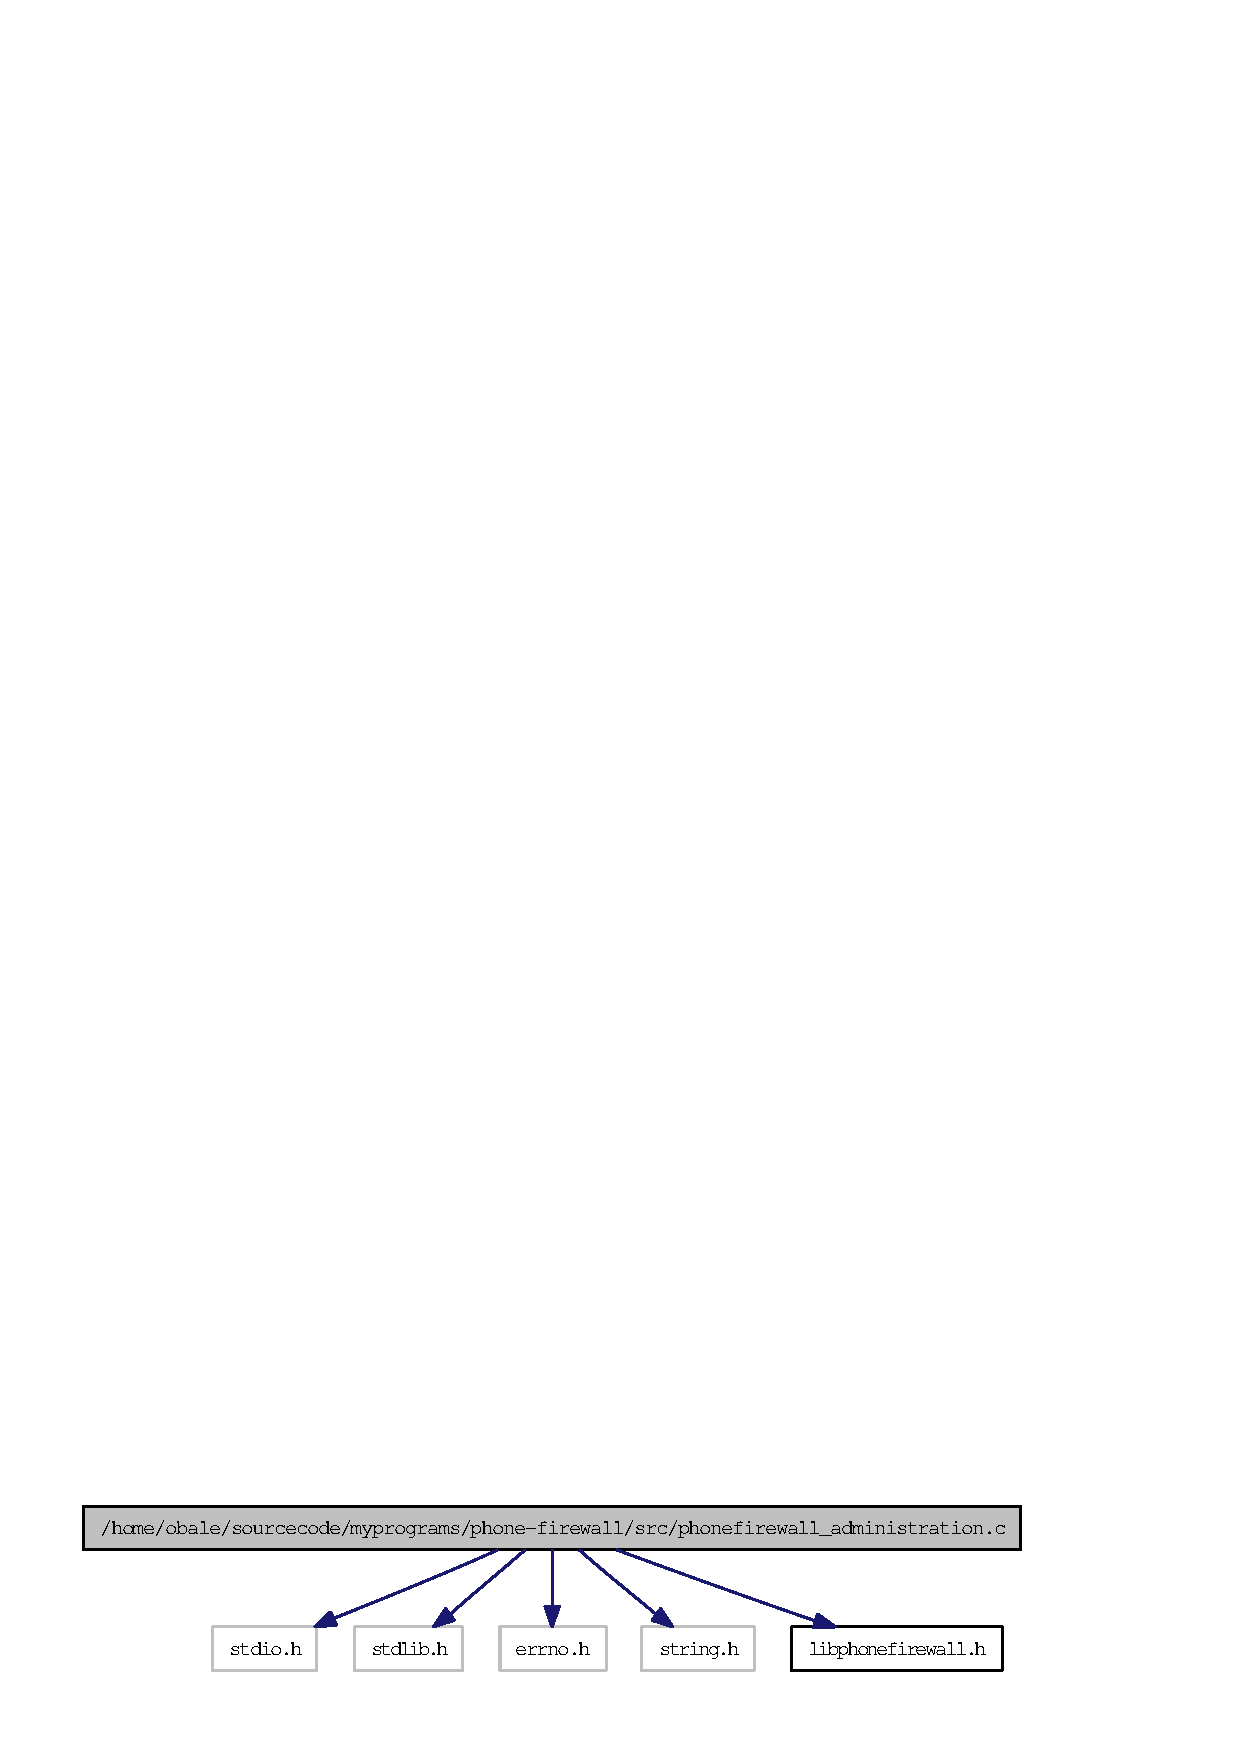
\includegraphics[width=211pt]{phonefirewall__administration_8c__incl}
\end{center}
\end{figure}
\subsection*{Defines}
\begin{CompactItemize}
\item 
\#define \hyperlink{phonefirewall__administration_8c_c0120f27d973f4ea90962305431fedce}{BLACKLIST\_\-PREFIX}~\char`\"{}db/blacklist\_\-\char`\"{}
\item 
\#define \hyperlink{phonefirewall__administration_8c_b5b8614b1e4d5e316cc4a8102ce9636c}{WHITELIST\_\-PREFIX}~\char`\"{}db/whitelist\_\-\char`\"{}
\item 
\#define \hyperlink{phonefirewall__administration_8c_03bc2a42c1399400ae0d103f5ada724c}{FILENAME\_\-SIZE}~256
\end{CompactItemize}
\subsection*{Functions}
\begin{CompactItemize}
\item 
int \hyperlink{phonefirewall__administration_8c_d42187af304bf25d98f7f7f76853c6f7}{set\_\-filename} (char $\ast$prefix, int country\_\-code, int area\_\-code)
\item 
int \hyperlink{phonefirewall__administration_8c_36847ed3459e2a89038772ece42a017d}{add\_\-blacklist\_\-entry} (int country\_\-code, int area\_\-code, unsigned long long number, char $\ast$name, char $\ast$reason, int priority)
\item 
int \hyperlink{phonefirewall__administration_8c_eec16cb88eb546b1a2490e6716d75f8b}{add\_\-whitelist\_\-entry} (int country\_\-code, int area\_\-code, unsigned long long number, char $\ast$name, char $\ast$reason, int priority)
\item 
int \hyperlink{phonefirewall__administration_8c_e6c567f38aaa0eaa9db3eb13e32cdbbd}{rm\_\-blacklist\_\-entry} (unsigned long long number)
\item 
int \hyperlink{phonefirewall__administration_8c_e8a4ee30cf26b05a55680dc3a972f1a4}{rm\_\-whitelist\_\-entry} (unsigned long long number)
\item 
char $\ast$ \hyperlink{phonefirewall__administration_8c_651cdd0245f20256305b40f13bb9df2d}{check\_\-blacklist\_\-entry} (int country\_\-code, int area\_\-code, unsigned long long number, int priority)
\item 
char $\ast$ \hyperlink{phonefirewall__administration_8c_032c45d6c7830492ddeaa8cabfc845c3}{check\_\-whitelist\_\-entry} (int country\_\-code, int area\_\-code, unsigned long long number, int priority)
\end{CompactItemize}
\subsection*{Variables}
\begin{CompactItemize}
\item 
static char $\ast$ \hyperlink{phonefirewall__administration_8c_6c7d3710dd8e86998206dad075d6fc27}{DELIM} = \char`\"{}::\char`\"{}
\item 
char \hyperlink{phonefirewall__administration_8c_89707f7a91e271cac7f8e4e2a0be0006}{filename} \mbox{[}FILENAME\_\-SIZE\mbox{]}
\end{CompactItemize}


\subsection{Define Documentation}
\hypertarget{phonefirewall__administration_8c_c0120f27d973f4ea90962305431fedce}{
\index{phonefirewall\_\-administration.c@{phonefirewall\_\-administration.c}!BLACKLIST\_\-PREFIX@{BLACKLIST\_\-PREFIX}}
\index{BLACKLIST\_\-PREFIX@{BLACKLIST\_\-PREFIX}!phonefirewall_administration.c@{phonefirewall\_\-administration.c}}
\subsubsection{\setlength{\rightskip}{0pt plus 5cm}\#define BLACKLIST\_\-PREFIX~\char`\"{}db/blacklist\_\-\char`\"{}}}
\label{phonefirewall__administration_8c_c0120f27d973f4ea90962305431fedce}




Definition at line 26 of file phonefirewall\_\-administration.c.

Referenced by add\_\-blacklist\_\-entry(), and check\_\-blacklist\_\-entry().\hypertarget{phonefirewall__administration_8c_03bc2a42c1399400ae0d103f5ada724c}{
\index{phonefirewall\_\-administration.c@{phonefirewall\_\-administration.c}!FILENAME\_\-SIZE@{FILENAME\_\-SIZE}}
\index{FILENAME\_\-SIZE@{FILENAME\_\-SIZE}!phonefirewall_administration.c@{phonefirewall\_\-administration.c}}
\subsubsection{\setlength{\rightskip}{0pt plus 5cm}\#define FILENAME\_\-SIZE~256}}
\label{phonefirewall__administration_8c_03bc2a42c1399400ae0d103f5ada724c}




Definition at line 28 of file phonefirewall\_\-administration.c.\hypertarget{phonefirewall__administration_8c_b5b8614b1e4d5e316cc4a8102ce9636c}{
\index{phonefirewall\_\-administration.c@{phonefirewall\_\-administration.c}!WHITELIST\_\-PREFIX@{WHITELIST\_\-PREFIX}}
\index{WHITELIST\_\-PREFIX@{WHITELIST\_\-PREFIX}!phonefirewall_administration.c@{phonefirewall\_\-administration.c}}
\subsubsection{\setlength{\rightskip}{0pt plus 5cm}\#define WHITELIST\_\-PREFIX~\char`\"{}db/whitelist\_\-\char`\"{}}}
\label{phonefirewall__administration_8c_b5b8614b1e4d5e316cc4a8102ce9636c}




Definition at line 27 of file phonefirewall\_\-administration.c.

Referenced by add\_\-whitelist\_\-entry(), and check\_\-whitelist\_\-entry().

\subsection{Function Documentation}
\hypertarget{phonefirewall__administration_8c_36847ed3459e2a89038772ece42a017d}{
\index{phonefirewall\_\-administration.c@{phonefirewall\_\-administration.c}!add\_\-blacklist\_\-entry@{add\_\-blacklist\_\-entry}}
\index{add\_\-blacklist\_\-entry@{add\_\-blacklist\_\-entry}!phonefirewall_administration.c@{phonefirewall\_\-administration.c}}
\subsubsection{\setlength{\rightskip}{0pt plus 5cm}int add\_\-blacklist\_\-entry (int {\em country\_\-code}, int {\em area\_\-code}, unsigned long long {\em number}, char $\ast$ {\em name}, char $\ast$ {\em reason}, int {\em priority})}}
\label{phonefirewall__administration_8c_36847ed3459e2a89038772ece42a017d}


Add a number to the blacklist. The number will be blocked after that.

\begin{Desc}
\item[Parameters:]
\begin{description}
\item[{\em country\_\-code}]The country code (for example 39 for Italy, 43 for Austria, and so one) \item[{\em area\_\-code}]The area code which indicates your mobile operator. \item[{\em number}]The telephone number of the person (without country and area code. \item[{\em name}]The name of the person. \item[{\em reason}]Why you have blocked this person. \item[{\em priority}]Gives the \hyperlink{structentry}{entry} a priority. 0 is standard. If the priority is higher the value will be also blocked/accepted if a higher priority is choosen.\end{description}
\end{Desc}
\begin{Desc}
\item[Returns:]If all goes well 0 (zero) otherwise an errno code. \end{Desc}


Definition at line 40 of file phonefirewall\_\-administration.c.

References BLACKLIST\_\-PREFIX, DELIM, filename, and set\_\-filename().

Here is the call graph for this function:\nopagebreak
\begin{figure}[H]
\begin{center}
\leavevmode
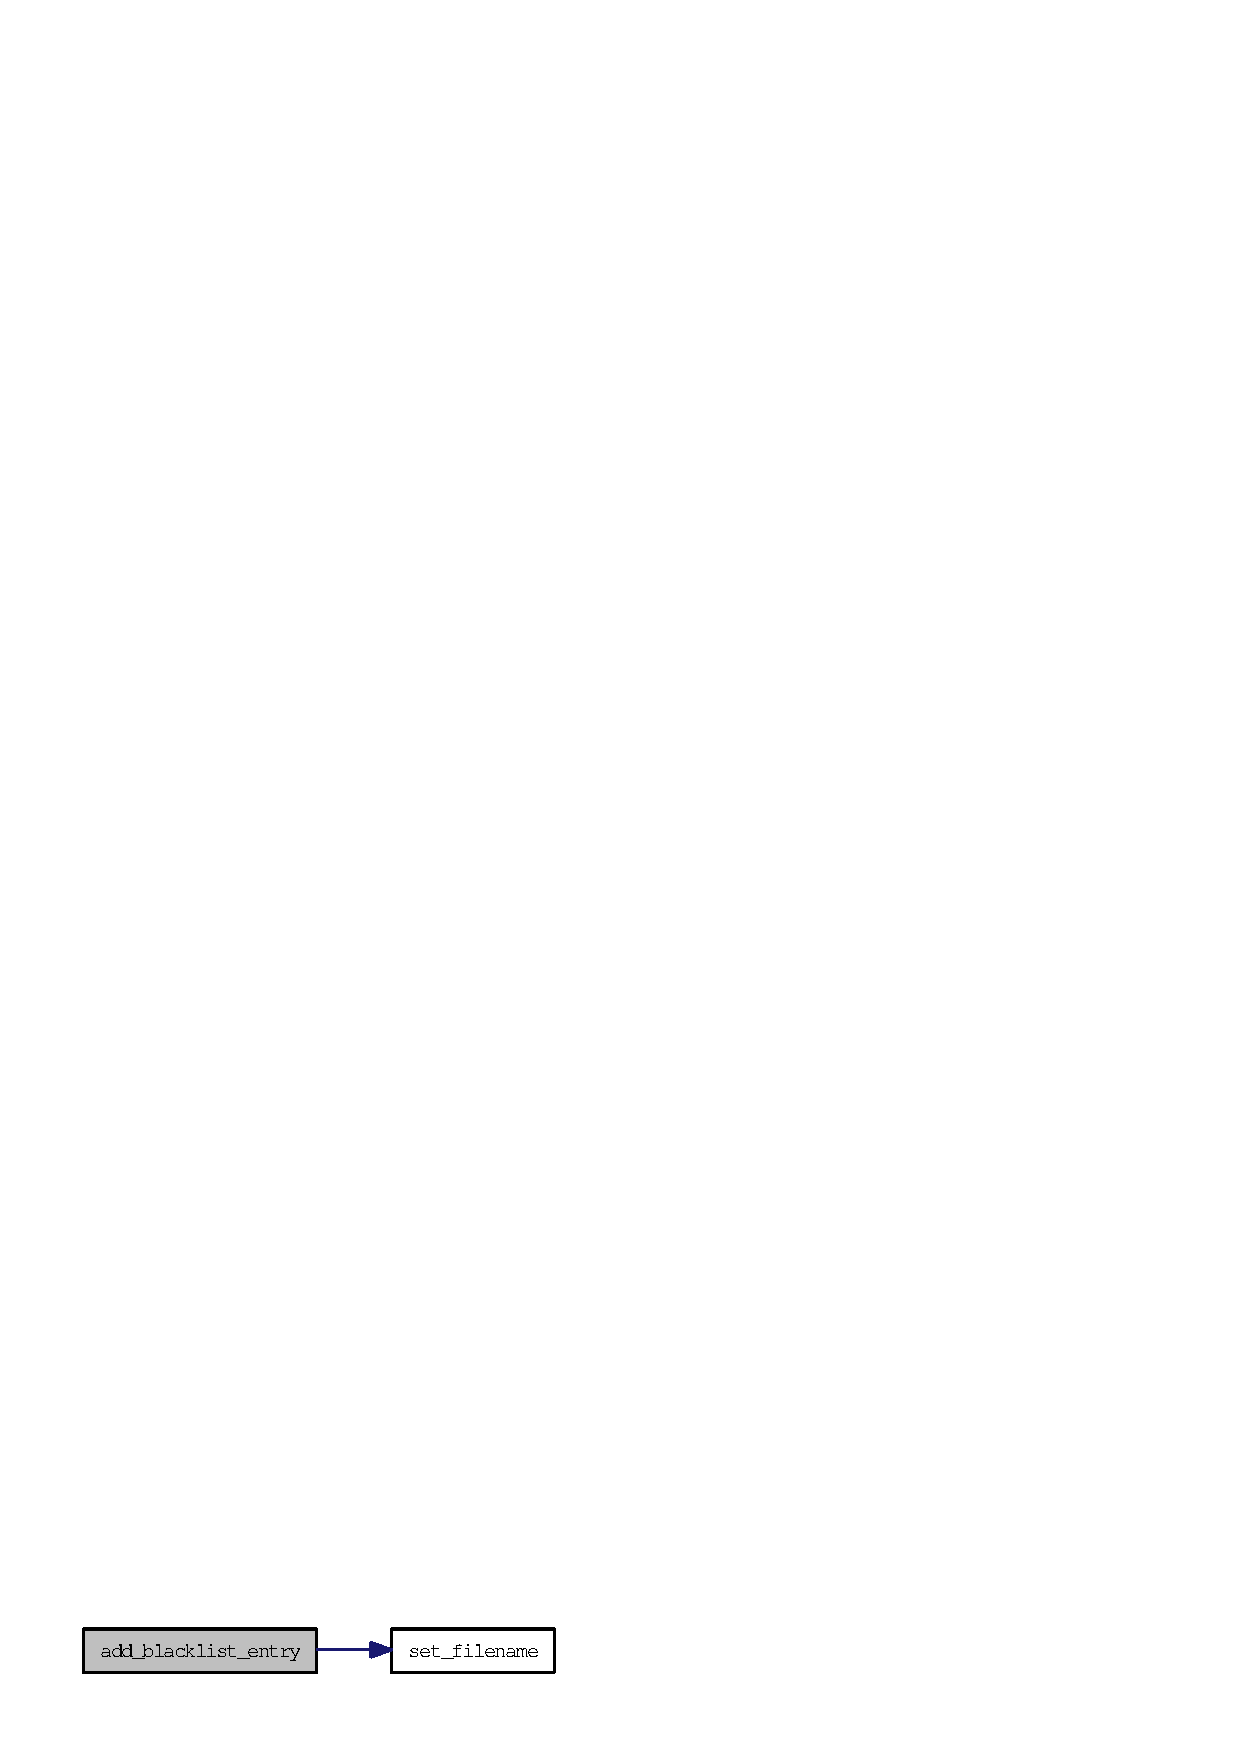
\includegraphics[width=135pt]{phonefirewall__administration_8c_36847ed3459e2a89038772ece42a017d_cgraph}
\end{center}
\end{figure}
\hypertarget{phonefirewall__administration_8c_eec16cb88eb546b1a2490e6716d75f8b}{
\index{phonefirewall\_\-administration.c@{phonefirewall\_\-administration.c}!add\_\-whitelist\_\-entry@{add\_\-whitelist\_\-entry}}
\index{add\_\-whitelist\_\-entry@{add\_\-whitelist\_\-entry}!phonefirewall_administration.c@{phonefirewall\_\-administration.c}}
\subsubsection{\setlength{\rightskip}{0pt plus 5cm}int add\_\-whitelist\_\-entry (int {\em country\_\-code}, int {\em area\_\-code}, unsigned long long {\em number}, char $\ast$ {\em name}, char $\ast$ {\em reason}, int {\em priority})}}
\label{phonefirewall__administration_8c_eec16cb88eb546b1a2490e6716d75f8b}


Add a number to the whitelist. The number will be accepted after that.

\begin{Desc}
\item[Parameters:]
\begin{description}
\item[{\em country\_\-code}]The country code (for example 39 for Italy, 43 for Austria, and so one) \item[{\em area\_\-code}]The area code which indicates your mobile operator. \item[{\em number}]The telephone number of the person (without country and area code. \item[{\em name}]The name of the person. \item[{\em reason}]Why you have blocked this person. \item[{\em priority}]Gives the \hyperlink{structentry}{entry} a priority. 0 is standard. If the priority is higher the value will be also blocked/accepted if a higher priority is choosen.\end{description}
\end{Desc}
\begin{Desc}
\item[Returns:]If all goes well 0 (zero) otherwise an errno code. \end{Desc}


Definition at line 54 of file phonefirewall\_\-administration.c.

References DELIM, filename, set\_\-filename(), and WHITELIST\_\-PREFIX.

Here is the call graph for this function:\nopagebreak
\begin{figure}[H]
\begin{center}
\leavevmode
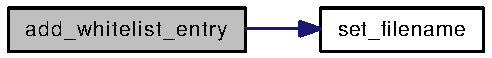
\includegraphics[width=136pt]{phonefirewall__administration_8c_eec16cb88eb546b1a2490e6716d75f8b_cgraph}
\end{center}
\end{figure}
\hypertarget{phonefirewall__administration_8c_651cdd0245f20256305b40f13bb9df2d}{
\index{phonefirewall\_\-administration.c@{phonefirewall\_\-administration.c}!check\_\-blacklist\_\-entry@{check\_\-blacklist\_\-entry}}
\index{check\_\-blacklist\_\-entry@{check\_\-blacklist\_\-entry}!phonefirewall_administration.c@{phonefirewall\_\-administration.c}}
\subsubsection{\setlength{\rightskip}{0pt plus 5cm}char$\ast$ check\_\-blacklist\_\-entry (int {\em country\_\-code}, int {\em area\_\-code}, unsigned long long {\em number}, int {\em priority})}}
\label{phonefirewall__administration_8c_651cdd0245f20256305b40f13bb9df2d}


Checks if a number is on the blacklist.

\begin{Desc}
\item[Parameters:]
\begin{description}
\item[{\em country\_\-code}]The country code (for example 39 for Italy, 43 for Austria, and so one) \item[{\em area\_\-code}]The area code which indicates your mobile operator. \item[{\em number}]The telephone number of the person (without country and area code. \item[{\em priority}]Gives the \hyperlink{structentry}{entry} a priority. 0 is standard. If the priority is higher the value will be also blocked/accepted if a higher priority is choosen.\end{description}
\end{Desc}
\begin{Desc}
\item[Returns:]If noting is found NULL, otherwise the number. \end{Desc}


Definition at line 76 of file phonefirewall\_\-administration.c.

References BLACKLIST\_\-PREFIX, DELIM, filename, MAX\_\-LINE\_\-LENGTH, and set\_\-filename().

Here is the call graph for this function:\nopagebreak
\begin{figure}[H]
\begin{center}
\leavevmode
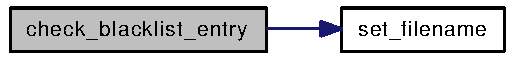
\includegraphics[width=141pt]{phonefirewall__administration_8c_651cdd0245f20256305b40f13bb9df2d_cgraph}
\end{center}
\end{figure}
\hypertarget{phonefirewall__administration_8c_032c45d6c7830492ddeaa8cabfc845c3}{
\index{phonefirewall\_\-administration.c@{phonefirewall\_\-administration.c}!check\_\-whitelist\_\-entry@{check\_\-whitelist\_\-entry}}
\index{check\_\-whitelist\_\-entry@{check\_\-whitelist\_\-entry}!phonefirewall_administration.c@{phonefirewall\_\-administration.c}}
\subsubsection{\setlength{\rightskip}{0pt plus 5cm}char$\ast$ check\_\-whitelist\_\-entry (int {\em country\_\-code}, int {\em area\_\-code}, unsigned long long {\em number}, int {\em priority})}}
\label{phonefirewall__administration_8c_032c45d6c7830492ddeaa8cabfc845c3}


Checks if a number is on the whitelist.

\begin{Desc}
\item[Parameters:]
\begin{description}
\item[{\em country\_\-code}]The country code (for example 39 for Italy, 43 for Austria, and so one) \item[{\em area\_\-code}]The area code which indicates your mobile operator. \item[{\em number}]The telephone number of the person (without country and area code. \item[{\em priority}]Gives the \hyperlink{structentry}{entry} a priority. 0 is standard. If the priority is higher the value will be also blocked/accepted if a higher priority is choosen.\end{description}
\end{Desc}
\begin{Desc}
\item[Returns:]If noting is found NULL, otherwise the number. \end{Desc}


Definition at line 110 of file phonefirewall\_\-administration.c.

References DELIM, filename, MAX\_\-LINE\_\-LENGTH, set\_\-filename(), and WHITELIST\_\-PREFIX.

Here is the call graph for this function:\nopagebreak
\begin{figure}[H]
\begin{center}
\leavevmode
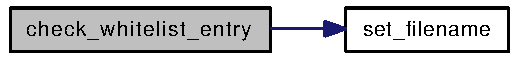
\includegraphics[width=142pt]{phonefirewall__administration_8c_032c45d6c7830492ddeaa8cabfc845c3_cgraph}
\end{center}
\end{figure}
\hypertarget{phonefirewall__administration_8c_e6c567f38aaa0eaa9db3eb13e32cdbbd}{
\index{phonefirewall\_\-administration.c@{phonefirewall\_\-administration.c}!rm\_\-blacklist\_\-entry@{rm\_\-blacklist\_\-entry}}
\index{rm\_\-blacklist\_\-entry@{rm\_\-blacklist\_\-entry}!phonefirewall_administration.c@{phonefirewall\_\-administration.c}}
\subsubsection{\setlength{\rightskip}{0pt plus 5cm}int rm\_\-blacklist\_\-entry (unsigned long long {\em number})}}
\label{phonefirewall__administration_8c_e6c567f38aaa0eaa9db3eb13e32cdbbd}


Removes a blocked number from the blacklist.

\begin{Desc}
\item[Parameters:]
\begin{description}
\item[{\em number}]The number which will be deleted.\end{description}
\end{Desc}
\begin{Desc}
\item[Returns:]If all goes right 0, otherwise an error code. \end{Desc}


Definition at line 68 of file phonefirewall\_\-administration.c.\hypertarget{phonefirewall__administration_8c_e8a4ee30cf26b05a55680dc3a972f1a4}{
\index{phonefirewall\_\-administration.c@{phonefirewall\_\-administration.c}!rm\_\-whitelist\_\-entry@{rm\_\-whitelist\_\-entry}}
\index{rm\_\-whitelist\_\-entry@{rm\_\-whitelist\_\-entry}!phonefirewall_administration.c@{phonefirewall\_\-administration.c}}
\subsubsection{\setlength{\rightskip}{0pt plus 5cm}int rm\_\-whitelist\_\-entry (unsigned long long {\em number})}}
\label{phonefirewall__administration_8c_e8a4ee30cf26b05a55680dc3a972f1a4}


Removes a accepted number from the whitelist.

\begin{Desc}
\item[Parameters:]
\begin{description}
\item[{\em number}]The number which will be deleted.\end{description}
\end{Desc}
\begin{Desc}
\item[Returns:]If all goes right 0, otherwise an error code. \end{Desc}


Definition at line 72 of file phonefirewall\_\-administration.c.\hypertarget{phonefirewall__administration_8c_d42187af304bf25d98f7f7f76853c6f7}{
\index{phonefirewall\_\-administration.c@{phonefirewall\_\-administration.c}!set\_\-filename@{set\_\-filename}}
\index{set\_\-filename@{set\_\-filename}!phonefirewall_administration.c@{phonefirewall\_\-administration.c}}
\subsubsection{\setlength{\rightskip}{0pt plus 5cm}int set\_\-filename (char $\ast$ {\em prefix}, int {\em country\_\-code}, int {\em area\_\-code})}}
\label{phonefirewall__administration_8c_d42187af304bf25d98f7f7f76853c6f7}




Definition at line 34 of file phonefirewall\_\-administration.c.

References filename.

Referenced by add\_\-blacklist\_\-entry(), add\_\-whitelist\_\-entry(), check\_\-blacklist\_\-entry(), and check\_\-whitelist\_\-entry().

Here is the caller graph for this function:\nopagebreak
\begin{figure}[H]
\begin{center}
\leavevmode
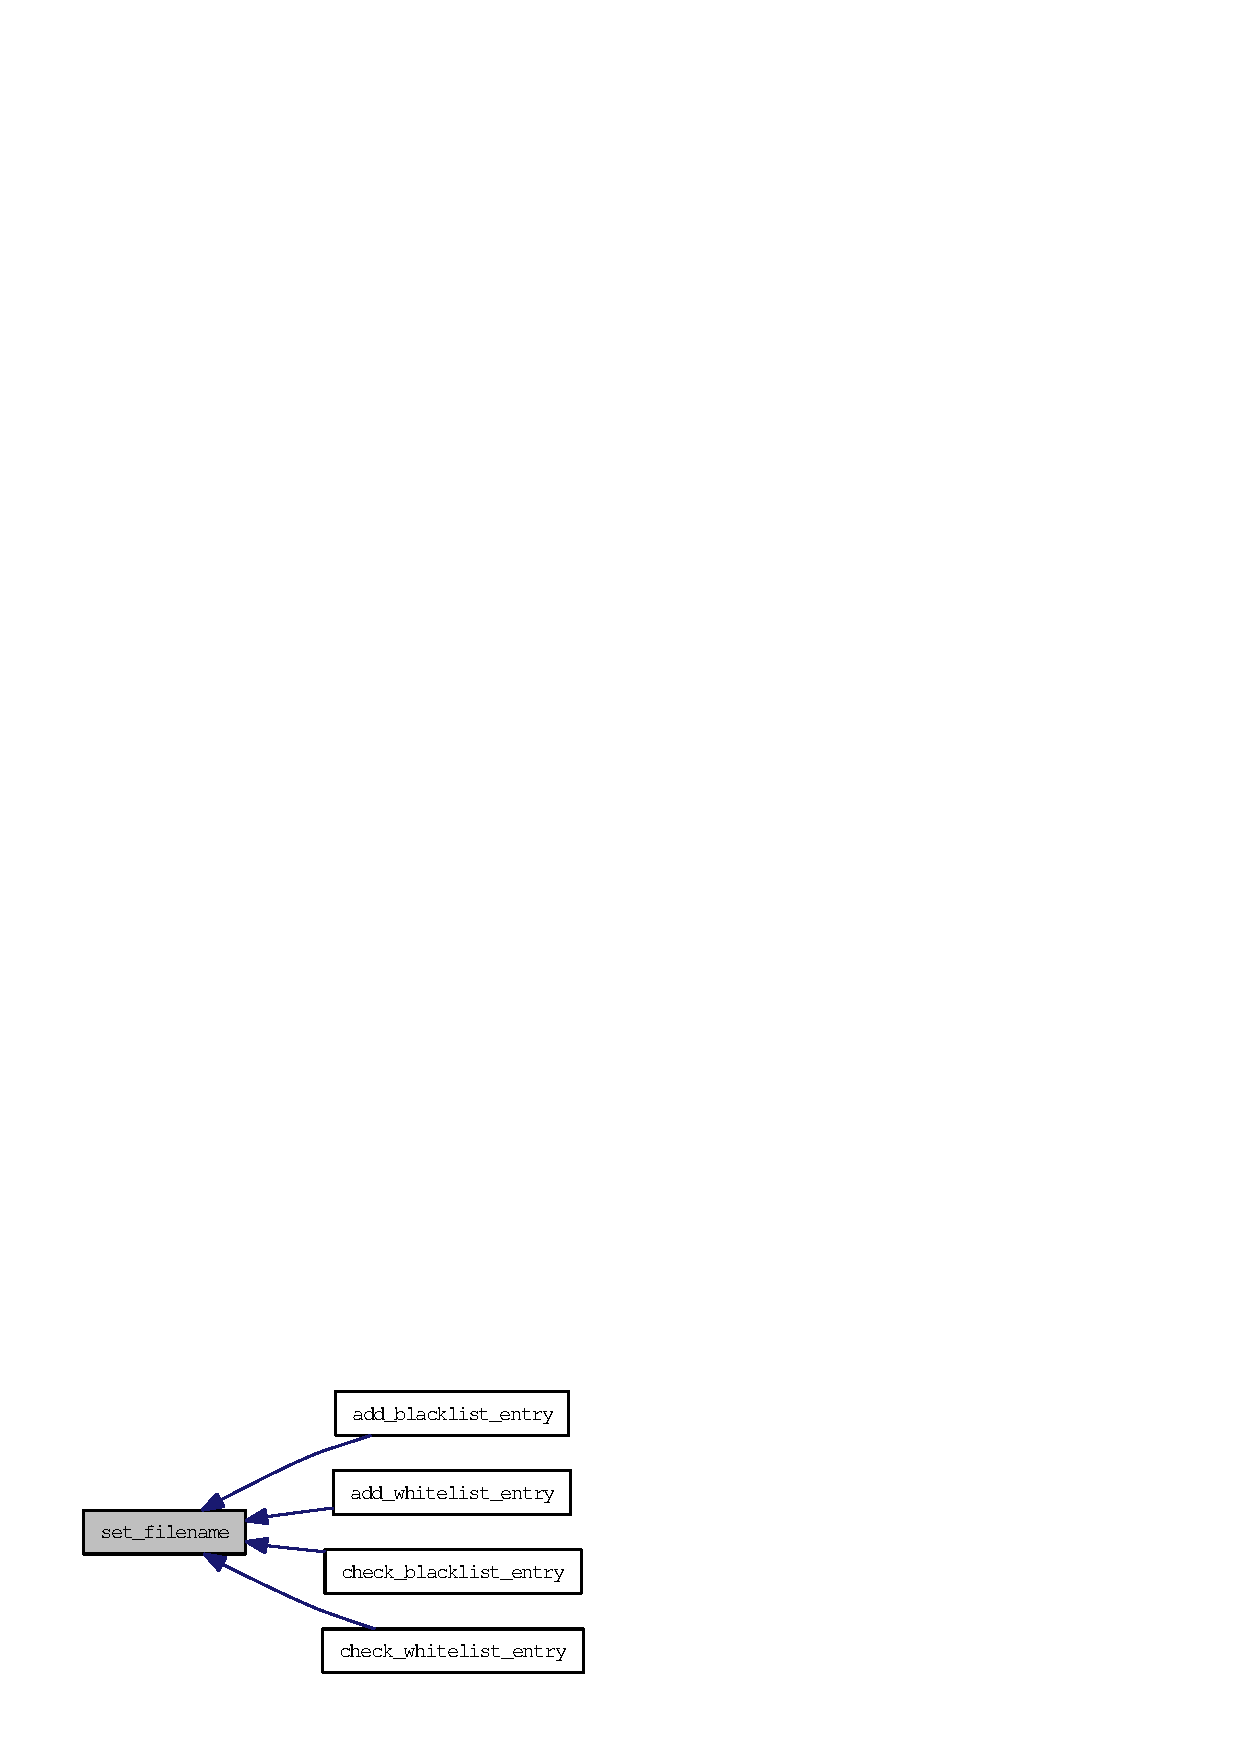
\includegraphics[width=142pt]{phonefirewall__administration_8c_d42187af304bf25d98f7f7f76853c6f7_icgraph}
\end{center}
\end{figure}


\subsection{Variable Documentation}
\hypertarget{phonefirewall__administration_8c_6c7d3710dd8e86998206dad075d6fc27}{
\index{phonefirewall\_\-administration.c@{phonefirewall\_\-administration.c}!DELIM@{DELIM}}
\index{DELIM@{DELIM}!phonefirewall_administration.c@{phonefirewall\_\-administration.c}}
\subsubsection{\setlength{\rightskip}{0pt plus 5cm}char$\ast$ {\bf DELIM} = \char`\"{}::\char`\"{}\hspace{0.3cm}{\tt  \mbox{[}static\mbox{]}}}}
\label{phonefirewall__administration_8c_6c7d3710dd8e86998206dad075d6fc27}




Definition at line 30 of file phonefirewall\_\-administration.c.

Referenced by add\_\-blacklist\_\-entry(), add\_\-whitelist\_\-entry(), check\_\-blacklist\_\-entry(), and check\_\-whitelist\_\-entry().\hypertarget{phonefirewall__administration_8c_89707f7a91e271cac7f8e4e2a0be0006}{
\index{phonefirewall\_\-administration.c@{phonefirewall\_\-administration.c}!filename@{filename}}
\index{filename@{filename}!phonefirewall_administration.c@{phonefirewall\_\-administration.c}}
\subsubsection{\setlength{\rightskip}{0pt plus 5cm}char {\bf filename}\mbox{[}FILENAME\_\-SIZE\mbox{]}}}
\label{phonefirewall__administration_8c_89707f7a91e271cac7f8e4e2a0be0006}




Definition at line 32 of file phonefirewall\_\-administration.c.

Referenced by add\_\-blacklist\_\-entry(), add\_\-whitelist\_\-entry(), check\_\-blacklist\_\-entry(), check\_\-whitelist\_\-entry(), and set\_\-filename().
\hypertarget{phonefirewall__search_8c}{
\section{phonefirewall\_\-search.c File Reference}
\label{phonefirewall__search_8c}\index{phonefirewall\_\-search.c@{phonefirewall\_\-search.c}}
}
{\tt \#include $<$stdio.h$>$}\par
{\tt \#include $<$stdlib.h$>$}\par
{\tt \#include $<$errno.h$>$}\par
{\tt \#include $<$string.h$>$}\par
{\tt \#include $<$sqlite3.h$>$}\par
{\tt \#include \char`\"{}libphonefirewall.h\char`\"{}}\par
{\tt \#include \char`\"{}logfile.h\char`\"{}}\par


Include dependency graph for phonefirewall\_\-search.c:\nopagebreak
\begin{figure}[H]
\begin{center}
\leavevmode
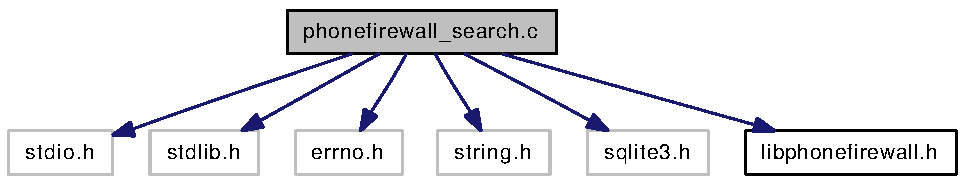
\includegraphics[width=279pt]{phonefirewall__search_8c__incl}
\end{center}
\end{figure}
\subsection*{Defines}
\begin{CompactItemize}
\item 
\#define \hyperlink{phonefirewall__search_8c_08df828ef9e922fa3a749f9bc0e4a42b}{ASCII\_\-PERCENT\_\-CHAR}~37
\item 
\#define \hyperlink{phonefirewall__search_8c_3b5bf1ced2c3343708fd193a487c2e26}{MAX\_\-ENTRY\_\-ARRAY}~1024
\end{CompactItemize}
\subsection*{Functions}
\begin{CompactItemize}
\item 
struct \hyperlink{structEntry}{Entry} $\ast$ \hyperlink{phonefirewall__search_8c_bc4a987c792bc712e4f1804a6f8be6b2}{find\_\-entry\_\-by\_\-name} (sqlite3\_\-stmt $\ast$pp\_\-stmt, char $\ast$name)
\item 
struct \hyperlink{structEntry}{Entry} $\ast$ \hyperlink{phonefirewall__search_8c_9d31efccbc01d9cef3876329cf9ed4a2}{get\_\-blacklist\_\-entry\_\-by\_\-name} (char $\ast$name)
\item 
struct \hyperlink{structEntry}{Entry} $\ast$ \hyperlink{phonefirewall__search_8c_f851d1fdef92a5442118f7bd19efde9e}{get\_\-blacklist\_\-entry\_\-by\_\-number} (int country\_\-code, int area\_\-code, unsigned long long number)
\item 
struct \hyperlink{structEntry}{Entry} $\ast$ \hyperlink{phonefirewall__search_8c_6a5f107f222114236b6374ef52300a98}{get\_\-whitelist\_\-entry\_\-by\_\-name} (char $\ast$name)
\item 
struct \hyperlink{structEntry}{Entry} $\ast$ \hyperlink{phonefirewall__search_8c_b1e42c1f4ad78b0666c44ac6b9047718}{get\_\-whitelist\_\-entry\_\-by\_\-number} (int country\_\-code, int area\_\-code, unsigned long long number)
\end{CompactItemize}
\subsection*{Variables}
\begin{CompactItemize}
\item 
struct \hyperlink{structEntry}{Entry} $\ast$ \hyperlink{phonefirewall__search_8c_6065da0f6097ff02236ecc4b7d04c912}{p\_\-entry} = \&\hyperlink{structentry}{entry}
\item 
struct \hyperlink{structEntry}{Entry} \hyperlink{phonefirewall__search_8c_4ac6231c71a3f59eeb4ae2462fb4dd54}{entry\_\-array} \mbox{[}MAX\_\-ENTRY\_\-ARRAY\mbox{]}
\end{CompactItemize}


\subsection{Define Documentation}
\hypertarget{phonefirewall__search_8c_08df828ef9e922fa3a749f9bc0e4a42b}{
\index{phonefirewall\_\-search.c@{phonefirewall\_\-search.c}!ASCII\_\-PERCENT\_\-CHAR@{ASCII\_\-PERCENT\_\-CHAR}}
\index{ASCII\_\-PERCENT\_\-CHAR@{ASCII\_\-PERCENT\_\-CHAR}!phonefirewall_search.c@{phonefirewall\_\-search.c}}
\subsubsection{\setlength{\rightskip}{0pt plus 5cm}\#define ASCII\_\-PERCENT\_\-CHAR~37}}
\label{phonefirewall__search_8c_08df828ef9e922fa3a749f9bc0e4a42b}




Definition at line 28 of file phonefirewall\_\-search.c.

Referenced by get\_\-blacklist\_\-entry\_\-by\_\-name().\hypertarget{phonefirewall__search_8c_3b5bf1ced2c3343708fd193a487c2e26}{
\index{phonefirewall\_\-search.c@{phonefirewall\_\-search.c}!MAX\_\-ENTRY\_\-ARRAY@{MAX\_\-ENTRY\_\-ARRAY}}
\index{MAX\_\-ENTRY\_\-ARRAY@{MAX\_\-ENTRY\_\-ARRAY}!phonefirewall_search.c@{phonefirewall\_\-search.c}}
\subsubsection{\setlength{\rightskip}{0pt plus 5cm}\#define MAX\_\-ENTRY\_\-ARRAY~1024}}
\label{phonefirewall__search_8c_3b5bf1ced2c3343708fd193a487c2e26}




Definition at line 29 of file phonefirewall\_\-search.c.

\subsection{Function Documentation}
\hypertarget{phonefirewall__search_8c_bc4a987c792bc712e4f1804a6f8be6b2}{
\index{phonefirewall\_\-search.c@{phonefirewall\_\-search.c}!find\_\-entry\_\-by\_\-name@{find\_\-entry\_\-by\_\-name}}
\index{find\_\-entry\_\-by\_\-name@{find\_\-entry\_\-by\_\-name}!phonefirewall_search.c@{phonefirewall\_\-search.c}}
\subsubsection{\setlength{\rightskip}{0pt plus 5cm}struct {\bf Entry}$\ast$ find\_\-entry\_\-by\_\-name (sqlite3\_\-stmt $\ast$ {\em pp\_\-stmt}, char $\ast$ {\em name})\hspace{0.3cm}{\tt  \mbox{[}read\mbox{]}}}}
\label{phonefirewall__search_8c_bc4a987c792bc712e4f1804a6f8be6b2}




Definition at line 34 of file phonefirewall\_\-search.c.

References Entry::area\_\-code, Entry::country\_\-code, Entry::name, Entry::number, Entry::priority, Entry::reason, TB\_\-AREACODE, TB\_\-COUNTRYCODE, TB\_\-NAME, TB\_\-NUMBER, TB\_\-PRIORITY, and TB\_\-REASON.

Referenced by get\_\-blacklist\_\-entry\_\-by\_\-name().

Here is the caller graph for this function:\nopagebreak
\begin{figure}[H]
\begin{center}
\leavevmode
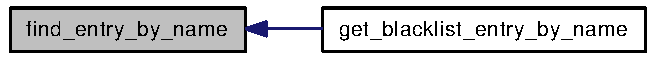
\includegraphics[width=175pt]{phonefirewall__search_8c_bc4a987c792bc712e4f1804a6f8be6b2_icgraph}
\end{center}
\end{figure}
\hypertarget{phonefirewall__search_8c_9d31efccbc01d9cef3876329cf9ed4a2}{
\index{phonefirewall\_\-search.c@{phonefirewall\_\-search.c}!get\_\-blacklist\_\-entry\_\-by\_\-name@{get\_\-blacklist\_\-entry\_\-by\_\-name}}
\index{get\_\-blacklist\_\-entry\_\-by\_\-name@{get\_\-blacklist\_\-entry\_\-by\_\-name}!phonefirewall_search.c@{phonefirewall\_\-search.c}}
\subsubsection{\setlength{\rightskip}{0pt plus 5cm}struct {\bf Entry}$\ast$ get\_\-blacklist\_\-entry\_\-by\_\-name (char $\ast$ {\em name})\hspace{0.3cm}{\tt  \mbox{[}read\mbox{]}}}}
\label{phonefirewall__search_8c_9d31efccbc01d9cef3876329cf9ed4a2}


Search a entrie by name.

\begin{Desc}
\item[Parameters:]
\begin{description}
\item[{\em name}]The name of the person which is blocked.\end{description}
\end{Desc}
\begin{Desc}
\item[Returns:]\hyperlink{structentry}{entry} Returns the found \hyperlink{structentry}{entry}. \end{Desc}


Definition at line 66 of file phonefirewall\_\-search.c.

References Entry::area\_\-code, ASCII\_\-PERCENT\_\-CHAR, Entry::country\_\-code, DB\_\-FILE, entry\_\-array, ERR\_\-FLAG, find\_\-entry\_\-by\_\-name(), MAX\_\-LINE\_\-LENGTH, Entry::number, Entry::reason, STMT\_\-SIZE, TB\_\-AREACODE, TB\_\-COUNTRYCODE, TB\_\-NAME, TB\_\-NUMBER, TB\_\-PRIORITY, TB\_\-REASON, and write\_\-logentry().

Here is the call graph for this function:\nopagebreak
\begin{figure}[H]
\begin{center}
\leavevmode
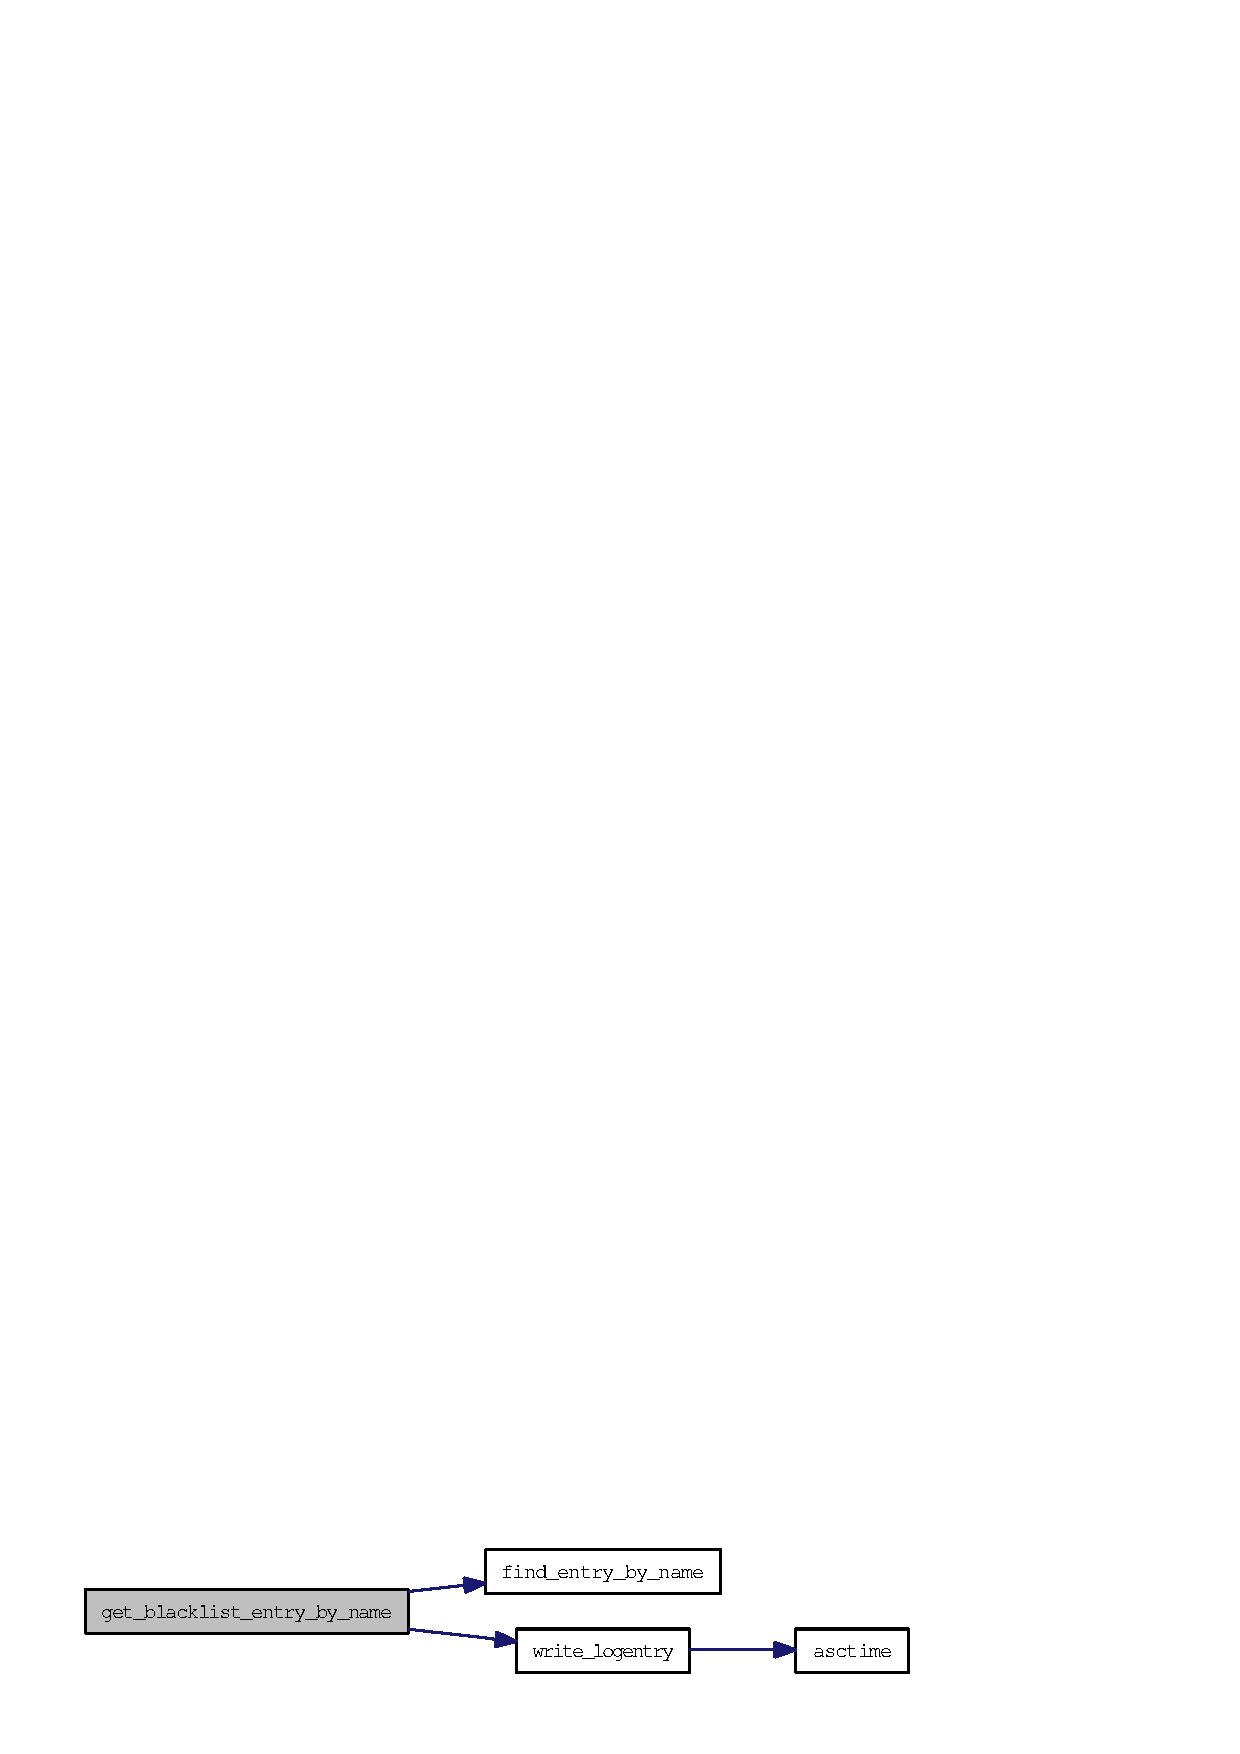
\includegraphics[width=220pt]{phonefirewall__search_8c_9d31efccbc01d9cef3876329cf9ed4a2_cgraph}
\end{center}
\end{figure}
\hypertarget{phonefirewall__search_8c_f851d1fdef92a5442118f7bd19efde9e}{
\index{phonefirewall\_\-search.c@{phonefirewall\_\-search.c}!get\_\-blacklist\_\-entry\_\-by\_\-number@{get\_\-blacklist\_\-entry\_\-by\_\-number}}
\index{get\_\-blacklist\_\-entry\_\-by\_\-number@{get\_\-blacklist\_\-entry\_\-by\_\-number}!phonefirewall_search.c@{phonefirewall\_\-search.c}}
\subsubsection{\setlength{\rightskip}{0pt plus 5cm}struct {\bf Entry}$\ast$ get\_\-blacklist\_\-entry\_\-by\_\-number (int {\em country\_\-code}, int {\em area\_\-code}, unsigned long long {\em number})\hspace{0.3cm}{\tt  \mbox{[}read\mbox{]}}}}
\label{phonefirewall__search_8c_f851d1fdef92a5442118f7bd19efde9e}


Search a entrie by number (country code + area code + number).

\begin{Desc}
\item[Parameters:]
\begin{description}
\item[{\em country\_\-code}]The country code (for example 39 for Italy, 43 for Austria, and so one) \item[{\em area\_\-code}]The area code which indicates your mobile operator. \item[{\em number}]The telephone number of the person (without country and area code.\end{description}
\end{Desc}
\begin{Desc}
\item[Returns:]\hyperlink{structentry}{entry} Returns the found \hyperlink{structentry}{entry}. \end{Desc}


Definition at line 115 of file phonefirewall\_\-search.c.\hypertarget{phonefirewall__search_8c_6a5f107f222114236b6374ef52300a98}{
\index{phonefirewall\_\-search.c@{phonefirewall\_\-search.c}!get\_\-whitelist\_\-entry\_\-by\_\-name@{get\_\-whitelist\_\-entry\_\-by\_\-name}}
\index{get\_\-whitelist\_\-entry\_\-by\_\-name@{get\_\-whitelist\_\-entry\_\-by\_\-name}!phonefirewall_search.c@{phonefirewall\_\-search.c}}
\subsubsection{\setlength{\rightskip}{0pt plus 5cm}struct {\bf Entry}$\ast$ get\_\-whitelist\_\-entry\_\-by\_\-name (char $\ast$ {\em name})\hspace{0.3cm}{\tt  \mbox{[}read\mbox{]}}}}
\label{phonefirewall__search_8c_6a5f107f222114236b6374ef52300a98}


Search a entrie by name.

\begin{Desc}
\item[Parameters:]
\begin{description}
\item[{\em name}]The name of the person which is accepted.\end{description}
\end{Desc}
\begin{Desc}
\item[Returns:]\hyperlink{structentry}{entry} Returns the found \hyperlink{structentry}{entry}. \end{Desc}


Definition at line 122 of file phonefirewall\_\-search.c.\hypertarget{phonefirewall__search_8c_b1e42c1f4ad78b0666c44ac6b9047718}{
\index{phonefirewall\_\-search.c@{phonefirewall\_\-search.c}!get\_\-whitelist\_\-entry\_\-by\_\-number@{get\_\-whitelist\_\-entry\_\-by\_\-number}}
\index{get\_\-whitelist\_\-entry\_\-by\_\-number@{get\_\-whitelist\_\-entry\_\-by\_\-number}!phonefirewall_search.c@{phonefirewall\_\-search.c}}
\subsubsection{\setlength{\rightskip}{0pt plus 5cm}struct {\bf Entry}$\ast$ get\_\-whitelist\_\-entry\_\-by\_\-number (int {\em country\_\-code}, int {\em area\_\-code}, unsigned long long {\em number})\hspace{0.3cm}{\tt  \mbox{[}read\mbox{]}}}}
\label{phonefirewall__search_8c_b1e42c1f4ad78b0666c44ac6b9047718}


Search a entrie by number (country code + area code + number).

\begin{Desc}
\item[Parameters:]
\begin{description}
\item[{\em country\_\-code}]The country code (for example 39 for Italy, 43 for Austria, and so one) \item[{\em area\_\-code}]The area code which indicates your mobile operator. \item[{\em number}]The telephone number of the person (without country and area code.\end{description}
\end{Desc}
\begin{Desc}
\item[Returns:]\hyperlink{structentry}{entry} Returns the found \hyperlink{structentry}{entry}. \end{Desc}


Definition at line 127 of file phonefirewall\_\-search.c.

\subsection{Variable Documentation}
\hypertarget{phonefirewall__search_8c_4ac6231c71a3f59eeb4ae2462fb4dd54}{
\index{phonefirewall\_\-search.c@{phonefirewall\_\-search.c}!entry\_\-array@{entry\_\-array}}
\index{entry\_\-array@{entry\_\-array}!phonefirewall_search.c@{phonefirewall\_\-search.c}}
\subsubsection{\setlength{\rightskip}{0pt plus 5cm}struct {\bf Entry} {\bf entry\_\-array}\mbox{[}MAX\_\-ENTRY\_\-ARRAY\mbox{]}}}
\label{phonefirewall__search_8c_4ac6231c71a3f59eeb4ae2462fb4dd54}




Definition at line 32 of file phonefirewall\_\-search.c.

Referenced by get\_\-blacklist\_\-entry\_\-by\_\-name().\hypertarget{phonefirewall__search_8c_6065da0f6097ff02236ecc4b7d04c912}{
\index{phonefirewall\_\-search.c@{phonefirewall\_\-search.c}!p\_\-entry@{p\_\-entry}}
\index{p\_\-entry@{p\_\-entry}!phonefirewall_search.c@{phonefirewall\_\-search.c}}
\subsubsection{\setlength{\rightskip}{0pt plus 5cm}struct {\bf Entry}$\ast$ {\bf p\_\-entry} = \&{\bf entry}}}
\label{phonefirewall__search_8c_6065da0f6097ff02236ecc4b7d04c912}




Definition at line 31 of file phonefirewall\_\-search.c.

Referenced by check\_\-blacklist\_\-entry(), and check\_\-whitelist\_\-entry().
\printindex
\end{document}
